% ============================================================
% SafeGuard - Safety Alert & Smart Protection System
% MCA Final Year Project Report
% ============================================================
%
% PROJECT DETAILS - UPDATE THESE VALUES:
%   <PROJECT TITLE>  -> SafeGuard --- Safety Alert \& Smart Protection System
%   <YOUR NAME>      -> Your full name
%   <YOUR USN>       -> Your USN/Roll Number
%   <COLLEGE NAME>   -> Your college name
%   <GUIDE NAME>     -> Your guide's name
%   <YEAR>           -> Academic year (e.g., 2025--2026)
%
% INSTRUCTIONS FOR OVERLEAF:
%   1. Upload all .tex files and references.bib to Overleaf
%   2. Ensure the file structure matches:
%      |-- main.tex
%      |-- preamble.tex
%      |-- references.bib
%      |-- frontmatter/
|      |   |-- titlepage.tex
%      |   |-- certificate.tex
%      |   |-- declaration.tex
%      |   |-- acknowledgement.tex
%      |   +-- abstract.tex
%      |-- chapters/
%      |   |-- chapter1.tex
%      |   |-- chapter2.tex
%      |   |-- chapter3.tex
%      |   |-- chapter4.tex
%      |   |-- chapter5.tex
%      |   |-- chapter6.tex
%      |   |-- chapter7.tex
%      |   +-- chapter8.tex
%      |-- backmatter/
%      |   +-- appendix.tex
%      +-- figures/
%          +-- (place screenshots here)
%
%   3. Set compiler to pdfLaTeX in Overleaf
%   4. Click Recompile
%
% ============================================================

\documentclass[12pt, a4paper, report]{report}

% Import preamble (packages and formatting)
% ============================================================
% PREAMBLE - Packages and Formatting
% ============================================================

% ----- Document Class -----
\documentclass[12pt, a4paper, report]{report}

% ----- Encoding and Language -----
\usepackage[utf8]{inputenc}
\usepackage[T1]{fontenc}
\usepackage[english]{babel}

% ----- Fonts -----
\usepackage{lmodern}
\usepackage{mathpazo}          % Palatino for a professional look

% ----- Page Layout -----
\usepackage[
  top=1in,
  bottom=1in,
  left=1.5in,
  right=1in,
  headheight=14pt
]{geometry}

% ----- Line Spacing -----
\usepackage{setspace}
\onehalfspacing

% ----- Headers and Footers -----
\usepackage{fancyhdr}
\pagestyle{fancy}
\fancyhf{}
\fancyhead[L]{\leftmark}
\fancyhead[R]{SafeGuard --- Safety Alert System}
\fancyfoot[C]{\thepage}
\renewcommand{\headrulewidth}{0.4pt}
\renewcommand{\footrulewidth}{0.4pt}

% Plain style for chapter pages
\fancypagestyle{plain}{
  \fancyhf{}
  \fancyfoot[C]{\thepage}
  \renewcommand{\headrulewidth}{0pt}
  \renewcommand{\footrulewidth}{0.4pt}
}

% ----- Mathematics -----
\usepackage{amsmath}
\usepackage{amssymb}

% ----- Graphics and Figures -----
\usepackage{graphicx}
\graphicspath{{figures/}{chapters/figures/}}
\usepackage{float}
\usepackage{caption}
\captionsetup{font=small, labelfont=bf, labelsep=period}
\usepackage{subcaption}

% ----- Tables -----
\usepackage{booktabs}
\usepackage{tabularx}
\usepackage{multirow}
\usepackage{array}
\usepackage{longtable}
\usepackage{colortbl}
\usepackage{xcolor}

% ----- Lists -----
\usepackage{enumitem}
\setlist{nosep, leftmargin=2cm}

% ----- Code Listings -----
\usepackage{listings}
\lstset{
  basicstyle=\ttfamily\small,
  breaklines=true,
  frame=single,
  numbers=left,
  numberstyle=\tiny\color{gray},
  keywordstyle=\color{blue},
  commentstyle=\color{green!50!black},
  stringstyle=\color{red!70!black},
  backgroundcolor=\color{gray!5},
  captionpos=b,
  tabsize=2,
  showstringspaces=false,
  morekeywords={self,cls,True,False,None,async,await,yield}
}

% ----- Diagrams with TikZ -----
\usepackage{tikz}
\usetikzlibrary{shapes, arrows.meta, positioning, calc, fit, backgrounds}
\usepackage{pgfplots}
\pgfplotsset{compat=1.18}

% ----- Hyperlinks -----
\usepackage[
  colorlinks=true,
  linkcolor=black,
  citecolor=blue!70!black,
  urlcolor=blue!70!black,
  bookmarks=true,
  pdfauthor={SafeGuard Project},
  pdftitle={Safety Alert \& Smart Protection System}
]{hyperref}

% ----- Bibliography -----
\usepackage[numbers, sort&compress]{natbib}
\bibliographystyle{unsrtnat}

% ----- Title Page -----
\usepackage{titling}

% ----- Chapter Styling -----
\usepackage{titlesec}
\titleformat{\chapter}[display]
  {\normalfont\huge\bfseries\centering}
  {Chapter \thechapter}
  {20pt}
  {\Huge}
\titlespacing*{\chapter}{0pt}{-30pt}{40pt}

% ----- Miscellaneous -----
\usepackage{lipsum}              % For placeholder if needed
\usepackage{setspace}
\usepackage{microtype}           % Microtypography
\usepackage{pdfpages}            % For including PDFs
\usepackage{rotating}            % For rotated tables/figures
\usepackage{acronym}             % For list of acronyms
\usepackage{appendix}            % For appendix support

% ----- Custom Commands -----
\newcommand{\projectTitle}{SafeGuard --- Safety Alert \& Smart Protection System}
\newcommand{\studentName}{\textit{<YOUR NAME>}}
\newcommand{\usnNumber}{\textit{<YOUR USN>}}
\newcommand{\collegeName}{\textit{<COLLEGE NAME>}}
\newcommand{\guideName}{\textit{<GUIDE NAME>}}
\newcommand{\academicYear}{\textit{2025--2026}}

% ----- Color Definitions -----
\definecolor{primaryblue}{RGB}{25, 118, 210}
\definecolor{darkgray}{RGB}{66, 66, 66}
\definecolor{lightgray}{RGB}{245, 245, 245}
\definecolor{sosred}{RGB}{211, 47, 47}

% ----- Placeholder Box Command -----
\newcommand{\placeholder}[2][0.4\textheight]{%
  \begin{figure}[H]
    \centering
    \fbox{\parbox{0.85\textwidth}{\centering\vspace{#1}%
      \textbf{[PLACEHOLDER: #2]}%
      \vspace{#1}}}
    \caption{#2}
    \label{fig:\refstepcounter{figure}\thefigure}
  \end{figure}
}

% ----- Table Placeholder -----
\newcommand{\tableplaceholder}[1]{%
  \vspace{0.5cm}
  \begin{center}
    \fbox{\parbox{0.8\textwidth}{\centering\vspace{2cm}%
      \textbf{[PLACEHOLDER: #1]}%
      \vspace{2cm}}}
  \end{center}
  \vspace{0.5cm}
}


% ============================================================
% BEGIN DOCUMENT
% ============================================================
\begin{document}

% ----- Front Matter -----
% Set page numbering to roman for front matter
\pagenumbering{roman}
\setcounter{page}{1}

% Title Page
% ============================================================
% TITLE PAGE
% ============================================================
\begin{titlepage}
  \begin{center}
    \vspace*{1cm}

    {\Large \textbf{\collegeName}}

    \vspace{0.5cm}
    {\large Department of Master of Computer Applications}

    \vspace{2cm}

    \rule{\textwidth}{1.5pt}

    \vspace{0.5cm}

    {\Huge \textbf{\projectTitle}}

    \vspace{0.5cm}

    \rule{\textwidth}{1.5pt}

    \vspace{2cm}

    {\Large \textbf{A Project Report}}

    \vspace{0.3cm}

    {\large Submitted in Partial Fulfilment of the Requirements\\
    for the Award of the Degree of}

    \vspace{0.5cm}

    {\Large \textbf{Master of Computer Applications (MCA)}}

    \vspace{2.5cm}

    \begin{minipage}{0.45\textwidth}
      \begin{flushleft}
        \textbf{Submitted By:}\\[0.3cm]
        \studentName\\
        USN: \usnNumber
      \end{flushleft}
    \end{minipage}
    \hfill
    \begin{minipage}{0.45\textwidth}
      \begin{flushright}
        \textbf{Guided By:}\\[0.3cm]
        \guideName\\
        Assistant Professor
      \end{flushleft}
    \end{minipage}

    \vfill

    {\large \textbf{Academic Year \academicYear}}

    \vspace{1cm}
  \end{center}
\end{titlepage}


% Certificate
% ============================================================
% CERTIFICATE
% ============================================================
\thispagestyle{plain}
\begin{center}
  \vspace*{1cm}
  {\Large \textbf{\collegeName}}\\[0.3cm]
  {\large Department of Master of Computer Applications}\\[2cm]
  {\LARGE \textbf{CERTIFICATE}}\\[1.5cm]
\end{center}

\begin{center}
  \begin{minipage}{0.9\textwidth}
    \setstretch{1.8}
    \large
    \noindent This is to certify that the project work entitled \textbf{``\projectTitle''} is a bonafide work carried out by \textbf{\studentName} bearing USN \textbf{\usnNumber} in partial fulfilment of the requirements for the award of the degree of \textbf{Master of Computer Applications (MCA)} from \collegeName.

    \vspace{1.5cm}

    \noindent The content embodied in this project report has not been submitted either in part or in full, for any other degree or diploma of this or any other institution or university.

    \vspace{3cm}

    \noindent\begin{minipage}{0.45\textwidth}
      \centering
      \rule{5cm}{0.5pt}\\
      \guideName\\
      (Project Guide)\\
      Assistant Professor\\
      Dept. of MCA\\
      \collegeName
    \end{minipage}
    \hfill
    \begin{minipage}{0.45\textwidth}
      \centering
      \rule{5cm}{0.5pt}\\
      Head of the Department\\
      Dept. of MCA\\
      \collegeName
    \end{minipage}

    \vspace{2cm}

    \noindent\begin{minipage}{0.45\textwidth}
      \centering
      \rule{5cm}{0.5pt}\\
      Principal\\
      \collegeName
    \end{minipage}
    \hfill
    \begin{minipage}{0.45\textwidth}
      \centering
      \vspace{1cm}
    \end{minipage}
  \end{minipage}
\end{center}


% Declaration
% ============================================================
% DECLARATION
% ============================================================
\thispagestyle{plain}
\begin{center}
  \vspace*{1cm}
  {\LARGE \textbf{DECLARATION}}\\[2cm]
\end{center}

\begin{center}
  \begin{minipage}{0.85\textwidth}
    \setstretch{1.8}
    \large

    \noindent I, \textbf{\studentName}, hereby declare that the project work entitled \textbf{``\projectTitle''} submitted to \collegeName, in partial fulfilment of the requirements for the award of the degree of \textbf{Master of Computer Applications (MCA)}, is a record of original work carried out by me under the guidance of \textbf{\guideName}, Assistant Professor, Department of Master of Computer Applications, \collegeName.

    \vspace{1cm}

    \noindent I further declare that the work embodied in this project report has not been submitted either in part or in full, for any other degree or diploma of this or any other institution or university. The project work has been carried out by me and has not been published anywhere.

    \vspace{1cm}

    \noindent The information and data presented in this report are authentic to the best of my knowledge. I further declare that I have duly acknowledged all the sources of information obtained from published and unpublished works.

    \vspace{3cm}

    \noindent\begin{minipage}{0.45\textwidth}
      \centering
      \rule{5cm}{0.5pt}\\
      \studentName\\
      USN: \usnNumber
    \end{minipage}
    \hfill
    \begin{minipage}{0.45\textwidth}
      \centering
      \rule{5cm}{0.5pt}\\
      Date:\\
      Place:
    \end{minipage}

  \end{minipage}
\end{center}


% Acknowledgement
% ============================================================
% ACKNOWLEDGEMENT
% ============================================================
\thispagestyle{plain}
\begin{center}
  \vspace*{1cm}
  {\LARGE \textbf{ACKNOWLEDGEMENT}}\\[2cm]
\end{center}

\begin{center}
  \begin{minipage}{0.85\textwidth}
    \setstretch{1.8}
    \large

    \noindent I would like to express my sincere gratitude to all those who have contributed to the successful completion of this project.

    \vspace{0.5cm}

    \noindent First and foremost, I am deeply grateful to Almighty God for granting me the strength, wisdom, and perseverance to complete this project successfully.

    \vspace{0.5cm}

    \noindent I extend my heartfelt thanks to \textbf{\guideName}, my project guide and Assistant Professor, Department of Master of Computer Applications, \collegeName, for his/her invaluable guidance, constant encouragement, and constructive suggestions throughout the course of this project. His/her expert knowledge and patient mentoring have been instrumental in shaping this work.

    \vspace{0.5cm}

    \noindent I express my sincere gratitude to \textbf{the Head of the Department}, Department of MCA, for providing the necessary infrastructure and support for carrying out this project.

    \vspace{0.5cm}

    \noindent I am also thankful to \textbf{the Principal}, \collegeName, for their encouragement and for providing me with the opportunity to pursue this academic endeavour.

    \vspace{0.5cm}

    \noindent I place on record my sincere appreciation to all the \textbf{faculty members} of the MCA department for their valuable teachings and support during my course of study. Their knowledge and dedication have laid the foundation for this project.

    \vspace{0.5cm}

    \noindent I am grateful to my \textbf{friends and classmates} who helped me with their suggestions, discussions, and moral support during the development of this project.

    \vspace{0.5cm}

    \noindent Finally, I express my deepest gratitude to my \textbf{parents and family members} for their unconditional love, support, and encouragement throughout my academic journey. Without their sacrifices and belief in my abilities, this project would not have been possible.

    \vspace{2cm}

    \noindent\begin{flushright}
      \rule{5cm}{0.5pt}\\
      \studentName\\
      USN: \usnNumber
    \end{flushright}

  \end{minipage}
\end{center}


% Abstract
% ============================================================
% ABSTRACT
% ============================================================
\thispagestyle{plain}
\begin{center}
  \vspace*{1cm}
  {\LARGE \textbf{ABSTRACT}}\\[2cm]
\end{center}

\begin{center}
  \begin{minipage}{0.85\textwidth}
    \setstretch{1.6}
    \large

    \noindent\textbf{Title:} \projectTitle

    \vspace{0.3cm}
    \noindent\textbf{Student:} \studentName \hfill \textbf{USN:} \usnNumber

    \vspace{0.3cm}
    \noindent\textbf{Guide:} \guideName

    \vspace{0.3cm}
    \noindent\textbf{Department:} Master of Computer Applications

    \vspace{0.3cm}
    \noindent\textbf{College:} \collegeName

    \vspace{1cm}

    \noindent Personal safety is a growing concern in modern society. Individuals frequently find themselves in situations where they need immediate assistance, yet lack a reliable and efficient mechanism to alert emergency contacts or authorities. Traditional safety systems are often fragmented, relying on separate applications for messaging, location sharing, and incident reporting, which leads to delayed responses and incomplete information during critical moments.

    \vspace{0.5cm}

    \noindent This project presents \textbf{SafeGuard}, a comprehensive Safety Alert and Smart Protection System designed as a full-stack web application. SafeGuard integrates multiple safety features into a single unified platform, enabling users to send SOS emergency alerts with real-time geolocation, manage a network of emergency contacts, and report and track safety incidents. The system is built using a modern three-tier architecture comprising React.js 18 with Material UI for the presentation layer, Python FastAPI for the application logic, and MySQL 8.0 with SQLAlchemy ORM for the data persistence layer.

    \vspace{0.5cm}

    \noindent The system provides six core functional modules: user authentication and profile management with JWT-based security, emergency contact management with priority-based classification, a one-press SOS emergency alerting mechanism with automatic geolocation capture, an incident reporting system with severity classification and status tracking, a comprehensive alert and incident history with CSV export capabilities, and a statistics dashboard providing real-time situational awareness.

    \vspace{0.5cm}

    \noindent SafeGuard addresses the critical need for an integrated personal safety platform that combines real-time emergency communication, location-aware alerting, and structured incident documentation. The system follows RESTful API design principles, implements robust security measures including bcrypt password hashing and JWT authentication, and ensures complete data isolation between users. The responsive dark/light themed user interface ensures accessibility across devices and user preferences.

    \vspace{0.5cm}

    \noindent The project demonstrates the effective application of modern web technologies, software engineering principles, and database design concepts to solve a real-world problem. Testing validates that all modules function correctly with acceptable response times, and the system meets its stated functional and non-functional requirements.

  \end{minipage}
\end{center}


% Table of Contents
\clearpage
\phantomsection
\addcontentsline{toc}{chapter}{Table of Contents}
\tableofcontents
\thispagestyle{plain}

% List of Figures
\clearpage
\phantomsection
\addcontentsline{toc}{chapter}{List of Figures}
\listoffigures
\thispagestyle{plain}

% List of Tables
\clearpage
\phantomsection
\addcontentsline{toc}{chapter}{List of Tables}
\listoftables
\thispagestyle{plain}

% Switch to arabic page numbering for main content
\clearpage
\pagenumbering{arabic}
\setcounter{page}{1}

% ============================================================
% MAIN CONTENT - CHAPTERS
% ============================================================

% Chapter 1: Introduction
% ============================================================
% CHAPTER 1: INTRODUCTION
% ============================================================
\chapter{Introduction}

\section{Introduction}

In an increasingly connected world, personal safety remains a fundamental concern for individuals across all demographics. The rapid proliferation of smartphones and wireless connectivity has created unprecedented opportunities to leverage technology for personal protection. However, despite the availability of numerous mobile applications and communication tools, there exists a significant gap in providing an integrated, reliable, and accessible platform for personal emergency management.

The Safety Alert and Smart Protection System, branded as \textbf{SafeGuard}, is conceived as a comprehensive web-based solution designed to bridge this gap. This system consolidates emergency alerting, contact management, incident reporting, and situational awareness into a unified platform accessible through any modern web browser. The project addresses the critical need for a centralized safety management system that can be relied upon during moments of distress, providing users with the tools necessary to quickly alert trusted contacts, document incidents, and maintain a chronological record of safety-related events.

This chapter provides an overview of the project, discusses the background and context in which it was developed, articulates the problem it addresses, examines existing solutions, and presents the proposed system along with its advantages.

\section{Background}

Personal safety technology has evolved significantly over the past two decades. Early emergency alert systems were primarily hardware-based, relying on dedicated devices such as personal emergency response systems (PERS) commonly used by elderly individuals. With the advent of smartphones, software-based solutions emerged, including mobile applications capable of sending SOS messages, sharing GPS coordinates, and triggering audible alarms~\cite{b2020mobile}.

Despite these advancements, existing solutions suffer from several limitations. Many applications are platform-specific, requiring installation on particular mobile operating systems. Others focus on a single aspect of safety, such as location sharing, without providing comprehensive incident documentation or contact management capabilities. Furthermore, the fragmented nature of the current ecosystem means that users often need multiple applications to cover different safety scenarios, leading to confusion and potential delays during emergencies~\cite{b2021smart}.

The emergence of modern web technologies, including progressive web applications (PWAs), real-time communication protocols, and geolocation APIs, has created new possibilities for building comprehensive safety platforms that transcend device and platform boundaries. The SafeGuard system leverages these technologies to deliver a cross-platform, feature-rich safety management solution.

\section{Problem Statement}

The core problem addressed by this project can be articulated as follows:

\begin{quote}
  \textit{``There is a need for an integrated, accessible, and reliable web-based personal safety management platform that enables individuals to send emergency alerts with real-time geolocation, manage emergency contacts, and systematically report and track safety incidents, all through a single unified interface.''}
\end{quote}

Specifically, the project addresses the following challenges:

\begin{enumerate}[label=\arabic*.]
  \item \textbf{Fragmentation of Safety Tools:} Current safety applications tend to focus on individual functionalities (messaging, location sharing, or incident reporting) rather than providing a holistic solution. Users must switch between multiple applications during emergencies, resulting in critical time loss.

  \item \textbf{Delayed Emergency Response:} In emergency situations, every second counts. Existing systems often require multiple steps to activate, and the lack of a streamlined SOS mechanism can delay the alerting of emergency contacts.

  \item \textbf{Inadequate Incident Documentation:} While some applications allow users to report incidents, few provide structured documentation with severity classification, status tracking, and chronological history, which are essential for follow-up actions and authorities.

  \item \textbf{Limited Accessibility:} Platform-specific applications exclude users who may not have access to compatible devices or prefer web-based solutions that do not require installation.

  \item \textbf{Lack of Integrated Geolocation:} Many safety systems do not effectively integrate real-time geolocation data with alerts and incident reports, reducing the situational awareness available to emergency contacts.
\end{enumerate}

\section{Existing System}

Several existing systems and applications attempt to address personal safety needs, each with varying degrees of success:

\begin{itemize}
  \item \textbf{Mobile SOS Applications:} Applications such as bSafe and Noonlight provide SOS alerting capabilities with location sharing. However, they are primarily mobile-native applications and lack comprehensive incident reporting and management dashboards.

  \item \textbf{Emergency Contact Services:} Services like ICE (In Case of Emergency) contacts stored in mobile phones provide basic emergency contact information but lack active alerting capabilities or incident tracking.

  \item \textbf{Government Emergency Systems:} Systems such as the Emergency Alert System (EAS) in the United States are designed for mass notifications and do not cater to individual personal safety needs.

  \item \textbf{Standalone Incident Reporting Tools:} Some platforms provide incident reporting but operate independently of alerting systems, requiring users to manually coordinate between tools.
\end{itemize}

The limitations of these existing systems include platform dependency, lack of integration between safety features, absence of structured incident management, and insufficient real-time geolocation capabilities.

\section{Proposed System}

The proposed system, \textbf{SafeGuard}, is a full-stack web application that integrates six core safety functionalities into a single cohesive platform:

\begin{enumerate}[label=\arabic*.]
  \item \textbf{User Authentication and Profile Management:} A secure registration and login system using JWT (JSON Web Token) authentication with bcrypt password hashing. Users can manage their profiles, upload profile pictures, and change passwords.

  \item \textbf{Emergency Contact Management:} A comprehensive contact management module enabling users to add, edit, search, and categorize emergency contacts with priority levels (low, medium, high, critical) and relationship types.

  \item \textbf{SOS Emergency Alert System:} A one-press SOS button that captures the user's real-time geolocation using the browser's Geolocation API and instantly notifies emergency contacts. The system supports multiple alert types including manual, automatic, panic, medical, fire, and security alerts.

  \item \textbf{Incident Reporting and Tracking:} A structured incident reporting module supporting eight incident types (theft, assault, accident, fire, harassment, vandalism, medical, other) with severity classification, geolocation tagging, image attachments, and status tracking through predefined stages (pending, investigating, resolved, closed).

  \item \textbf{Alert and Incident History:} A unified history view with tabbed navigation, multi-criteria filtering, search capabilities, and CSV export functionality for record-keeping and analysis.

  \item \textbf{Statistics Dashboard:} A real-time dashboard providing summary statistics, recent alerts, recent incidents, and activity logs, offering users immediate situational awareness.
\end{enumerate}

The system is built on a modern three-tier architecture:

\begin{itemize}
  \item \textbf{Presentation Tier:} React.js 18 with Material UI 5, featuring responsive design, dark/light theme support, and component-based architecture.
  \item \textbf{Application Tier:} Python FastAPI framework implementing RESTful APIs with dependency injection, Pydantic validation, and async request handling.
  \item \textbf{Data Tier:} MySQL 8.0 relational database with five normalized tables managed through SQLAlchemy ORM.
\end{itemize}

\section{Advantages of the Proposed System}

The SafeGuard system offers several significant advantages over existing solutions:

\begin{enumerate}[label=\arabic*.]
  \item \textbf{Platform Independence:} As a web application, SafeGuard is accessible from any device with a modern web browser, eliminating platform-specific dependencies.

  \item \textbf{Integrated Solution:} By consolidating alerting, contact management, incident reporting, and history tracking into a single platform, SafeGuard eliminates the need for multiple applications.

  \item \textbf{Rapid SOS Activation:} The one-press SOS button with automatic geolocation capture ensures that emergency alerts can be sent within seconds, minimizing response time.

  \item \textbf{Structured Incident Management:} The incident reporting system provides comprehensive documentation with severity levels, status tracking, and image attachments, supporting effective follow-up and record-keeping.

  \item \textbf{Data Isolation and Security:} Each user's data is completely isolated, with JWT authentication, password hashing, and per-user query filtering ensuring robust security.

  \item \textbf{Real-Time Situational Awareness:} The dashboard provides immediate visibility into recent alerts, incidents, and activities, enabling informed decision-making.

  \item \textbf{Scalable Architecture:} The decoupled frontend-backend architecture using RESTful APIs enables independent scaling and development of each tier.

  \item \textbf{Responsive Design:} The Material UI-based interface adapts seamlessly to desktop, tablet, and mobile devices, ensuring accessibility across screen sizes.

  \item \textbf{Dark/Light Theme Support:} Built-in theme management with localStorage persistence caters to user preferences and accessibility requirements.

  \item \textbf{Export Capabilities:} The CSV export feature enables users to download their alert and incident history for offline analysis, printing, or submission to authorities.
\end{enumerate}


% Chapter 2: Objectives and Scope
% ============================================================
% CHAPTER 2: OBJECTIVES AND SCOPE
% ============================================================
\chapter{Objectives and Scope}

\section{Project Objectives}

The primary objective of the SafeGuard project is to design, develop, and deploy a comprehensive web-based personal safety management system. The specific objectives of the project are as follows:

\begin{enumerate}[label=\textbf{O\arabic*.}]
  \item \textbf{Design a Secure Authentication System:} To implement a robust user authentication mechanism using JWT (JSON Web Token) technology with bcrypt password hashing, ensuring secure access to the platform and protection of user credentials.

  \item \textbf{Develop an Emergency Contact Management Module:} To create a functional module that allows users to maintain a structured network of emergency contacts with associated metadata including relationship type, priority level, and multiple communication channels.

  \item \textbf{Implement a Real-Time SOS Alerting Mechanism:} To build an SOS emergency alert system that captures real-time geolocation data through the browser's Geolocation API and facilitates immediate notification of emergency contacts with customizable alert messages.

  \item \textbf{Create a Structured Incident Reporting System:} To develop an incident reporting module supporting multiple incident types, severity classification, geolocation tagging, evidence attachment, and lifecycle status tracking.

  \item \textbf{Build a Unified History and Analytics Dashboard:} To provide users with a comprehensive dashboard displaying aggregated statistics, recent activities, and historical records with filtering, search, and export capabilities.

  \item \textbf{Ensure Cross-Platform Accessibility:} To deliver a responsive web application accessible across devices and browsers, eliminating platform-specific dependencies through progressive enhancement.

  \item \textbf{Apply Modern Software Engineering Practices:} To demonstrate the application of industry-standard practices including RESTful API design, three-tier architecture, ORM-based data access, component-based UI development, and security best practices.
\end{enumerate}

\section{Scope}

\subsection{In Scope}

The scope of the SafeGuard project encompasses the following functional areas:

\begin{itemize}
  \item User registration, login, and profile management with JWT authentication
  \item Password change and profile picture upload functionality
  \item Emergency contact CRUD (Create, Read, Update, Delete) operations
  \item Contact search and priority-based filtering
  \item SOS alert creation with geolocation capture and multiple alert types
  \item SOS alert history with pagination, search, and status filtering
  \item Incident reporting with type classification, severity levels, and location data
  \item Incident status tracking through pending, investigating, resolved, and closed stages
  \item Incident image upload and attachment
  \item Combined alert and incident history with tabbed navigation
  \item CSV export of SOS alerts and incident records
  \item Statistics dashboard with aggregated metrics and recent activity feeds
  \item Activity logging for significant user actions
  \item Dark and light theme support with persistence
  \item Responsive design for desktop and mobile devices
  \item Role-based access control foundation (user and admin roles)
\end{itemize}

\subsection{Out of Scope}

The following features and functionalities are explicitly outside the scope of this project:

\begin{itemize}
  \item Real-time push notifications to emergency contacts via SMS or email
  \item Integration with third-party emergency services (police, ambulance, fire department)
  \item Video or voice calling capabilities
  \item Map-based visualization of alerts and incidents (GIS integration)
  \item Mobile native applications (iOS or Android)
  \item Multi-language (internationalization) support
  \item Offline data synchronization and caching
  \item Advanced analytics and machine learning-based threat detection
  \item Multi-factor authentication (MFA)
  \item Social media integration and sharing
\end{itemize}

\section{Applications}

The SafeGuard system has potential applications across several domains:

\begin{enumerate}[label=\arabic*.]
  \item \textbf{Personal Safety:} Individuals can use the platform to manage their personal safety, quickly alert trusted contacts during emergencies, and maintain a record of safety incidents.

  \item \textbf{Campus Security:} Educational institutions can deploy the system for students and staff, enabling centralized incident reporting and emergency communication.

  \item \textbf{Workplace Safety:} Organizations can utilize the platform for employee safety management, particularly for employees working in high-risk environments or field operations.

  \item \textbf{Travel Safety:} Travelers can use the system to maintain emergency contacts across locations and report incidents while travelling.

  \item \textbf{Community Safety:} Community organizations can leverage the platform for neighbourhood watch programs and community-based safety initiatives.
\end{enumerate}

\section{Benefits}

The SafeGuard project delivers benefits at multiple levels:

\subsection{User Benefits}
\begin{itemize}
  \item Single-platform solution for all personal safety needs
  \item Rapid emergency alerting with automatic location sharing
  \item Organized emergency contact management with priority classification
  \item Structured incident documentation for personal records and legal proceedings
  \item Accessibility from any device with a web browser
  \item Intuitive and aesthetically pleasing user interface
  \item Privacy through complete data isolation between users
\end{itemize}

\subsection{Technical Benefits}
\begin{itemize}
  \item Modern technology stack ensuring long-term maintainability
  \item RESTful API architecture enabling future integration with mobile applications
  \item Component-based frontend enabling rapid feature development
  \item Database normalization ensuring data integrity and efficient queries
  \item Security best practices including password hashing and token-based authentication
  \item Scalable architecture supporting horizontal and vertical scaling
\end{itemize}

\subsection{Academic Benefits}
\begin{itemize}
  \item Demonstrates application of full-stack web development concepts
  \item Applies database design and normalization principles
  \item Implements software engineering methodologies including requirements analysis, system design, and testing
  \item Provides practical experience with industry-standard frameworks and tools
\end{itemize}

\section{Limitations}

Despite its comprehensive feature set, the SafeGuard system has certain limitations:

\begin{enumerate}[label=\arabic*.]
  \item \textbf{Internet Dependency:} As a web application, SafeGuard requires an active internet connection to function. It does not support offline operation or data synchronization.

  \item \textbf{No Real-Time Notification Delivery:} The system records SOS alerts but does not actively push notifications to emergency contacts via SMS, email, or push notifications. Contacts must be manually notified.

  \item \textbf{No Native Mobile App:} The application is web-based and does not provide native mobile applications, which may limit accessibility in low-connectivity scenarios.

  \item \textbf{Geolocation Accuracy:} The accuracy of geolocation data depends on the device's GPS capabilities and may be limited indoors or in areas with poor satellite visibility.

  \item \textbf{Single-User Focus:} The current implementation focuses on individual personal safety and does not support group safety management or organizational deployment.

  \item \textbf{No Integration with Emergency Services:} The system does not integrate with police, ambulance, or fire department dispatch systems, limiting its utility in critical emergencies.

  \item \textbf{Limited Admin Functionality:} While the database schema supports admin roles, the current implementation provides limited administrative features for system management.

  \item \textbf{No Multi-Factor Authentication:} The authentication system relies solely on JWT tokens and does not implement multi-factor authentication for additional security.
\end{enumerate}


% Chapter 3: System Analysis and Design
% ============================================================
% CHAPTER 3: SYSTEM ANALYSIS AND DESIGN
% ============================================================
\chapter{System Analysis and Design}

This chapter presents a detailed analysis and design of the SafeGuard system. It covers the functional and non-functional requirements, system architecture, UML design diagrams, and module descriptions that collectively define the system's structure and behaviour.

\section{Functional Requirements}

The functional requirements of the SafeGuard system are organized by module and specify the behaviours and capabilities the system must provide.

\subsection{User Authentication Module}

\begin{table}[H]
  \centering
  \caption{Functional Requirements: User Authentication}
  \label{tab:fr-auth}
  \begin{tabularx}{\textwidth}{@{}l l X@{}}
    \toprule
    \textbf{ID} & \textbf{Requirement} & \textbf{Description} \\
    \midrule
    FR-AUTH-01 & User Registration & The system shall allow new users to register by providing first name, last name, email address, phone number, password, and password confirmation. The system shall validate email uniqueness and password strength. \\
    FR-AUTH-02 & User Login & The system shall authenticate users using email address and password. Upon successful authentication, the system shall issue a JWT access token valid for 24 hours. \\
    FR-AUTH-03 & Password Hashing & The system shall hash all passwords using bcrypt before storage. Plain-text passwords shall never be stored in the database. \\
    FR-AUTH-04 & Session Management & The system shall use JWT Bearer tokens for session management. Tokens shall be attached to requests via the Authorization header. \\
    FR-AUTH-05 & Auto-Logout & The system shall automatically log out users when their token expires or when a 401 Unauthorized response is received from the server. \\
    FR-AUTH-06 & Profile Management & The system shall allow authenticated users to view and update their profile information, including name, email, and phone number. \\
    FR-AUTH-07 & Password Change & The system shall allow users to change their password by verifying the current password before accepting the new password. \\
    FR-AUTH-08 & Profile Picture & The system shall allow users to upload a profile picture in JPEG, PNG, or WebP format with a maximum size of 5MB. \\
    \bottomrule
  \end{tabularx}
\end{table}

\subsection{Emergency Contact Module}

\begin{table}[H]
  \centering
  \caption{Functional Requirements: Emergency Contacts}
  \label{tab:fr-contacts}
  \begin{tabularx}{\textwidth}{@{}l l X@{}}
    \toprule
    \textbf{ID} & \textbf{Requirement} & \textbf{Description} \\
    \midrule
    FR-CON-01 & Add Contact & The system shall allow users to add emergency contacts with name, relationship, phone number, email (optional), and priority level. \\
    FR-CON-02 & View Contacts & The system shall display all emergency contacts in a card-based layout with avatar initials and contact details. \\
    FR-CON-03 & Edit Contact & The system shall allow users to modify all fields of an existing emergency contact. \\
    FR-CON-04 & Delete Contact & The system shall allow users to remove an emergency contact with a confirmation dialog. \\
    FR-CON-05 & Search Contacts & The system shall provide search functionality across name, phone, and relationship fields using case-insensitive matching. \\
    FR-CON-06 & Priority Filter & The system shall allow filtering contacts by priority level (low, medium, high, critical). \\
    FR-CON-07 & Priority Levels & The system shall support four priority levels: low, medium, high, and critical, with appropriate visual indicators. \\
    \bottomrule
  \end{tabularx}
\end{table}

\subsection{SOS Alert Module}

\begin{table}[H]
  \centering
  \caption{Functional Requirements: SOS Alert System}
  \label{tab:fr-sos}
  \begin{tabularx}{\textwidth}{@{}l l X@{}}
    \toprule
    \textbf{ID} & \textbf{Requirement} & \textbf{Description} \\
    \midrule
    FR-SOS-01 & SOS Trigger & The system shall provide a prominent SOS button that triggers an emergency alert upon confirmation. \\
    FR-SOS-02 & Geolocation & The system shall automatically capture the user's current latitude and longitude using the browser Geolocation API when an SOS is triggered. \\
    FR-SOS-03 & Alert Types & The system shall support six alert types: manual, automatic, panic, medical, fire, and security. \\
    FR-SOS-04 & Custom Message & The system shall allow users to include a custom message with their SOS alert. \\
    FR-SOS-05 & Alert Status & The system shall track alert status through four states: active, acknowledged, resolved, and cancelled. \\
    FR-SOS-06 & Alert History & The system shall maintain a paginated history of all SOS alerts with filtering by status and search. \\
    FR-SOS-07 & Activity Logging & The system shall log every SOS alert trigger in the activity log with timestamp and details. \\
    \bottomrule
  \end{tabularx}
\end{table}

\subsection{Incident Reporting Module}

\begin{table}[H]
  \centering
  \caption{Functional Requirements: Incident Reporting}
  \label{tab:fr-incident}
  \begin{tabularx}{\textwidth}{@{}l l X@{}}
    \toprule
    \textbf{ID} & \textbf{Requirement} & \textbf{Description} \\
    \midrule
    FR-INC-01 & Report Incident & The system shall allow users to report incidents with type, description, location, severity, and optional image attachment. \\
    FR-INC-02 & Incident ID & The system shall auto-generate a unique incident identifier in the format INC-XXXXXXXX for each report. \\
    FR-INC-03 & Incident Types & The system shall support eight incident types: theft, assault, accident, fire, harassment, vandalism, medical, and other. \\
    FR-INC-04 & Severity Levels & The system shall classify incidents by severity: low, medium, high, and critical. \\
    FR-INC-05 & Status Tracking & The system shall track incident status through: pending, investigating, resolved, and closed. \\
    FR-INC-06 & Geolocation & The system shall support latitude and longitude coordinates for incident location. \\
    FR-INC-07 & Search and Filter & The system shall provide multi-criteria filtering by type, severity, status, and text search. \\
    FR-INC-08 & CRUD Operations & The system shall support creating, viewing, editing, and deleting incident reports. \\
    \bottomrule
  \end{tabularx}
\end{table}

\subsection{Dashboard Module}

\begin{table}[H]
  \centering
  \caption{Functional Requirements: Dashboard}
  \label{tab:fr-dashboard}
  \begin{tabularx}{\textwidth}{@{}l l X@{}}
    \toprule
    \textbf{ID} & \textbf{Requirement} & \textbf{Description} \\
    \midrule
    FR-DASH-01 & Statistics Cards & The system shall display summary statistics: total contacts, total SOS alerts, active SOS alerts, and total incidents. \\
    FR-DASH-02 & Recent Alerts & The system shall display the five most recent SOS alerts with status indicators. \\
    FR-DASH-03 & Recent Incidents & The system shall display the five most recent incidents with severity indicators. \\
    FR-DASH-04 & Activity Log & The system shall display the five most recent activity log entries. \\
    FR-DASH-05 & Quick SOS & The system shall provide a quick-access SOS button on the dashboard. \\
    \bottomrule
  \end{tabularx}
\end{table}

\section{Non-Functional Requirements}

\begin{table}[H]
  \centering
  \caption{Non-Functional Requirements}
  \label{tab:nfr}
  \begin{tabularx}{\textwidth}{@{}l l X@{}}
    \toprule
    \textbf{ID} & \textbf{Category} & \textbf{Requirement} \\
    \midrule
    NFR-01 & Performance & The system shall respond to user interactions within 2 seconds under normal load conditions. \\
    NFR-02 & Security & All passwords shall be hashed using bcrypt with salt. JWT tokens shall expire after 24 hours. \\
    NFR-03 & Data Isolation & Each user shall have access only to their own data. Cross-user data access shall be prevented at the API level. \\
    NFR-04 & Usability & The interface shall be intuitive, requiring no more than 3 clicks to reach any primary feature. \\
    NFR-05 & Accessibility & The system shall provide dark and light themes to accommodate user preferences and accessibility needs. \\
    NFR-06 & Compatibility & The system shall function on modern browsers including Chrome, Firefox, Safari, and Edge. \\
    NFR-07 & Scalability & The decoupled architecture shall support independent scaling of frontend and backend components. \\
    NFR-08 & Reliability & The system shall handle errors gracefully with appropriate user feedback messages. \\
    NFR-09 & Maintainability & The codebase shall follow modular architecture with clear separation of concerns. \\
    NFR-10 & File Security & Uploaded files shall be validated for type and size before storage. Maximum file size: 5MB. \\
    \bottomrule
  \end{tabularx}
\end{table}

\section{System Architecture}

The SafeGuard system follows a classic three-tier architecture with clear separation between the presentation, application, and data tiers. Figure~\ref{fig:architecture} illustrates the high-level system architecture.

\begin{figure}[H]
  \centering
  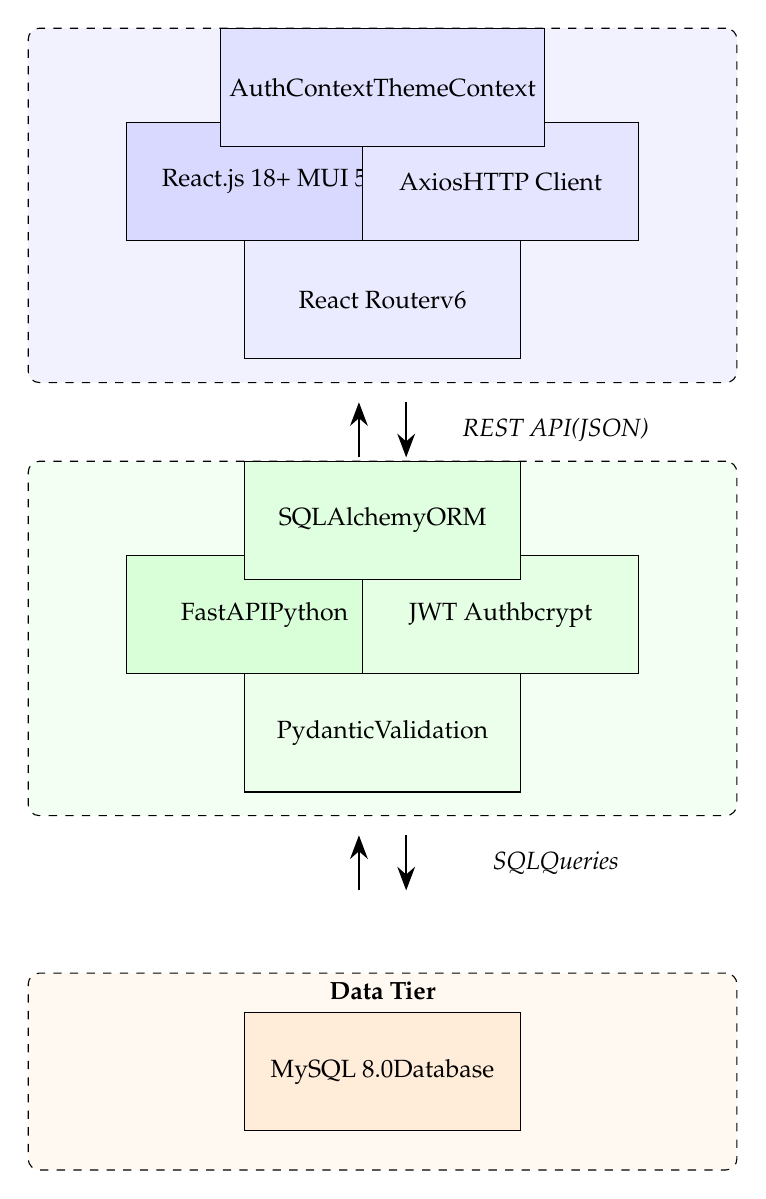
\begin{tikzpicture}[
    box/.style={rectangle, draw, minimum width=3.5cm, minimum height=1.5cm, text centered, font=\small},
    arrow/.style={-{Stealth[length=3mm]}, thick},
    label/.style={font=\small\itshape},
    tierbox/.style={rectangle, draw, dashed, rounded corners, inner sep=10pt}
  ]

    % Presentation Tier
    \begin{scope}[xshift=0cm]
      \node[tierbox, minimum width=9cm, minimum height=4.5cm, fill=blue!5] (ptier) at (0,0) {};
      \node[font=\small\bfseries, anchor=north] at (ptier.north) {Presentation Tier};
      \node[box, fill=blue!15] (react) at (-1.5, 0.3) {React.js 18\\+ MUI 5};
      \node[box, fill=blue!10] (axios) at (1.5, 0.3) {Axios\\HTTP Client};
      \node[box, fill=blue!8] (router) at (0, -1.2) {React Router\\v6};
      \node[box, fill=blue!12] (ctx) at (0, 1.5) {AuthContext\\ThemeContext};
    \end{scope}

    % Arrow
    \draw[arrow] (0.3, -2.5) -- (0.3, -3.2);
    \draw[arrow] (-0.3, -3.2) -- (-0.3, -2.5);
    \node[label] at (2.2, -2.85) {REST API\\(JSON)};

    % Application Tier
    \begin{scope}[xshift=0cm, yshift=-5.5cm]
      \node[tierbox, minimum width=9cm, minimum height=4.5cm, fill=green!5] (atier) at (0,0) {};
      \node[font=\small\bfseries, anchor=north] at (atier.north) {Application Tier};
      \node[box, fill=green!15] (fastapi) at (-1.5, 0.3) {FastAPI\\Python};
      \node[box, fill=green!10] (auth) at (1.5, 0.3) {JWT Auth\\bcrypt};
      \node[box, fill=green!8] (pydantic) at (0, -1.2) {Pydantic\\Validation};
      \node[box, fill=green!12] (sa) at (0, 1.5) {SQLAlchemy\\ORM};
    \end{scope}

    % Arrow
    \draw[arrow] (0.3, -8) -- (0.3, -8.7);
    \draw[arrow] (-0.3, -8.7) -- (-0.3, -8);
    \node[label] at (2.2, -8.35) {SQL\\Queries};

    % Data Tier
    \begin{scope}[xshift=0cm, yshift=-11cm]
      \node[tierbox, minimum width=9cm, minimum height=2.5cm, fill=orange!5] (dtier) at (0,0) {};
      \node[font=\small\bfseries, anchor=north] at (dtier.north) {Data Tier};
      \node[box, fill=orange!15] (mysql) at (0, 0) {MySQL 8.0\\Database};
    \end{scope}

  \end{tikzpicture}
  \caption{Three-Tier System Architecture}
  \label{fig:architecture}
\end{figure}

\subsection{Presentation Tier}

The presentation tier is implemented using React.js 18, a declarative, component-based JavaScript library for building user interfaces. Material UI 5 provides the component library for consistent and professional UI elements. The tier includes:

\begin{itemize}
  \item \textbf{React Router v6} for client-side routing with route guards
  \item \textbf{Context API} for global state management (authentication and theme)
  \item \textbf{Axios} for HTTP communication with request/response interceptors
  \item \textbf{Emotion} for CSS-in-JS styling
\end{itemize}

\subsection{Application Tier}

The application tier is implemented using Python's FastAPI framework, chosen for its automatic request validation, dependency injection system, and native async support. Key components include:

\begin{itemize}
  \item \textbf{FastAPI Router} for organizing API endpoints by module
  \item \textbf{Pydantic Schemas} for request/response validation and serialization
  \item \textbf{JWT Authentication} using python-jose for token generation and validation
  \item \textbf{bcrypt} for password hashing with salting
  \item \textbf{SQLAlchemy ORM} for database-agnostic data access
\end{itemize}

\subsection{Data Tier}

The data tier uses MySQL 8.0 as the relational database management system, accessed through SQLAlchemy ORM with PyMySQL as the database driver. The schema consists of five normalized tables with proper foreign key relationships and cascade delete rules.

\section{Use Case Diagram}

Figure~\ref{fig:usecase} presents the use case diagram for the SafeGuard system, illustrating the interactions between the actor (User) and the system's primary use cases.

\begin{figure}[H]
  \centering
  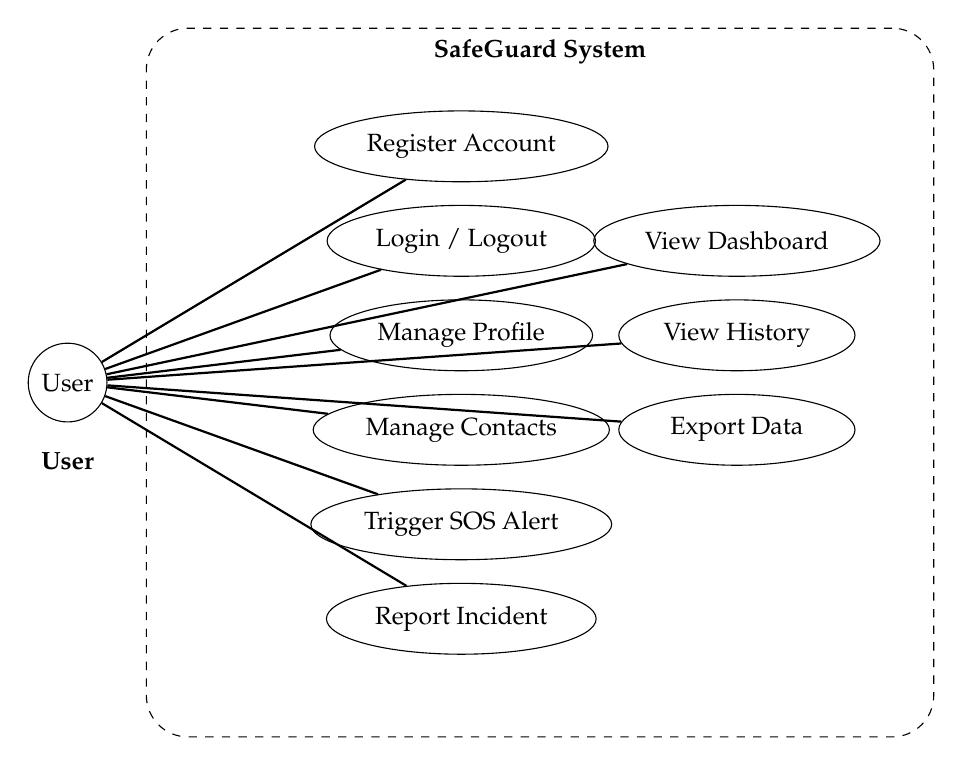
\begin{tikzpicture}[
    actor/.style={circle, draw, minimum size=1cm, inner sep=0pt, font=\small},
    usecase/.style={ellipse, draw, minimum width=3cm, minimum height=0.9cm, text centered, font=\small},
    system/.style={rectangle, draw, dashed, rounded corners=15pt, minimum width=10cm, minimum height=9cm},
    line/.style={thick}
  ]

    % System boundary
    \node[system] (sys) at (5.5,0) {};
    \node[font=\small\bfseries] at (5.5, 4.2) {SafeGuard System};

    % Actor
    \node[actor] (user) at (-0.5, 0) {User};
    \node[font=\small] at (-0.5, -1) {\textbf{User}};

    % Use cases
    \node[usecase] (uc1) at (4.5, 3) {Register Account};
    \node[usecase] (uc2) at (4.5, 1.8) {Login / Logout};
    \node[usecase] (uc3) at (4.5, 0.6) {Manage Profile};
    \node[usecase] (uc4) at (4.5, -0.6) {Manage Contacts};
    \node[usecase] (uc5) at (4.5, -1.8) {Trigger SOS Alert};
    \node[usecase] (uc6) at (4.5, -3.0) {Report Incident};
    \node[usecase] (uc7) at (8, 1.8) {View Dashboard};
    \node[usecase] (uc8) at (8, 0.6) {View History};
    \node[usecase] (uc9) at (8, -0.6) {Export Data};

    % Lines
    \draw[line] (user) -- (uc1);
    \draw[line] (user) -- (uc2);
    \draw[line] (user) -- (uc3);
    \draw[line] (user) -- (uc4);
    \draw[line] (user) -- (uc5);
    \draw[line] (user) -- (uc6);
    \draw[line] (user) -- (uc7);
    \draw[line] (user) -- (uc8);
    \draw[line] (user) -- (uc9);

  \end{tikzpicture}
  \caption{Use Case Diagram}
  \label{fig:usecase}
\end{figure}

\section{Activity Diagram}

Figure~\ref{fig:activity-sos} illustrates the activity flow when a user triggers an SOS alert, representing one of the most critical workflows in the system.

\begin{figure}[H]
  \centering
  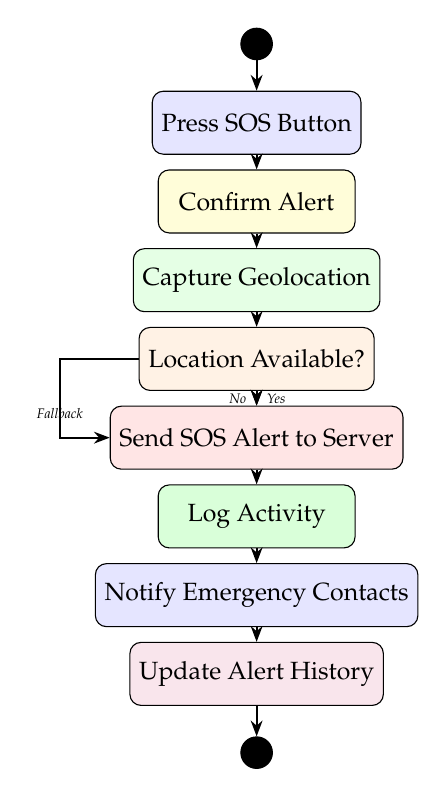
\begin{tikzpicture}[
    activity/.style={rectangle, rounded corners, draw, minimum width=2.5cm, minimum height=0.8cm, text centered, font=\small},
    decision/.style={diamond, draw, minimum size=1.5cm, text centered, font=\small},
    startend/.style={circle, draw, fill=black, minimum size=0.4cm, inner sep=0pt},
    flow/.style={-{Stealth[length=2mm]}, thick},
    yesno/.style={font=\tiny\itshape}
  ]

    % Start
    \node[startend] (start) at (0, 5) {};

    % Activities
    \node[activity, fill=blue!10] (press) at (0, 4) {Press SOS Button};
    \node[activity, fill=yellow!15] (confirm) at (0, 3) {Confirm Alert};
    \node[activity, fill=green!10] (geo) at (0, 2) {Capture Geolocation};
    \node[activity, fill=orange!10] (check) at (0, 1) {Location Available?};
    \node[activity, fill=red!10] (send) at (0, 0) {Send SOS Alert to Server};
    \node[activity, fill=green!15] (log) at (0, -1) {Log Activity};
    \node[activity, fill=blue!10] (notify) at (0, -2) {Notify Emergency Contacts};
    \node[activity, fill=purple!10] (update) at (0, -3) {Update Alert History};
    \node[startend] (end) at (0, -4) {};

    % Flows
    \draw[flow] (start) -- (press);
    \draw[flow] (press) -- (confirm);
    \draw[flow] (confirm) -- (geo);
    \draw[flow] (geo) -- (check);
    \draw[flow] (check) -- node[yesno, right] {Yes} (send);
    \draw[flow] (check) -- node[yesno, left] {No} (send);
    \draw[flow] (send) -- (log);
    \draw[flow] (log) -- (notify);
    \draw[flow] (notify) -- (update);
    \draw[flow] (update) -- (end);

    % Bypass path from check to send
    \draw[flow] (check.west) -- ++(-1,0) |- node[yesno, near start, below] {Fallback} (send.west);

  \end{tikzpicture}
  \caption{Activity Diagram: SOS Alert Workflow}
  \label{fig:activity-sos}
\end{figure}

\section{Sequence Diagram}

Figure~\ref{fig:sequence-login} depicts the sequence diagram for the user login process, illustrating the interaction between the user, frontend, backend API, and database.

\begin{figure}[H]
  \centering
  \begin{tikzpicture}[
    participant/.style={rectangle, draw, minimum width=2cm, minimum height=0.8cm, text centered, font=\small},
    message/.style={-{Stealth[length=2mm]}, thick},
    selfmsg/.style={thick, decorate, decoration={snake, amplitude=1mm, segment length=3mm}},
    returnmsg/.style={-{Stealth[length=2mm]}, thick, dashed},
    lifeline/.style={dashed, gray},
    xstart=-1.5, gap=3.5
  ]

    % Participants
    \node[participant, fill=blue!10] (user) at (0, 5) {User};
    \node[participant, fill=green!10] (fe) at (3.5, 5) {React Frontend};
    \node[participant, fill=orange!10] (api) at (7, 5) {FastAPI Backend};
    \node[participant, fill=red!10] (db) at (10.5, 5) {MySQL DB};

    % Lifelines
    \draw[lifeline] (user) -- (0, -3);
    \draw[lifeline] (fe) -- (3.5, -3);
    \draw[lifeline] (api) -- (7, -3);
    \draw[lifeline] (db) -- (10.5, -3);

    % Messages
    \draw[message] (0, 4) -- node[above, font=\tiny] {1. Enter credentials} (3.5, 4);
    \draw[message] (3.5, 3.3) -- node[above, font=\tiny] {2. POST /api/login} (7, 3.3);
    \draw[message] (7, 2.6) -- node[above, font=\tiny] {3. SELECT user by email} (10.5, 2.6);
    \draw[returnmsg] (10.5, 2) -- node[below, font=\tiny] {4. User record} (7, 2);
    \draw[message] (7, 1.3) -- node[above, font=\tiny] {5. Verify bcrypt hash} (7, 1.3) edge[selfloop, looseness=10, in=200, out=160, distance=1cm];
    \draw[message] (7, 0.6) -- node[above, font=\tiny] {6. Log activity} (10.5, 0.6);
    \draw[message] (10.5, 0) -- node[above, font=\tiny] {7. INSERT activity log} (10.5, 0) edge[selfloop, looseness=10, in=340, out=20, distance=0.8cm];
    \draw[returnmsg] (7, -0.5) -- node[below, font=\tiny] {8. JWT token + user} (3.5, -0.5);
    \draw[returnmsg] (3.5, -1.2) -- node[below, font=\tiny] {9. Store token, redirect} (0, -1.2);

  \end{tikzpicture}
  \caption{Sequence Diagram: User Login Process}
  \label{fig:sequence-login}
\end{figure}

\section{Class Diagram}

Figure~\ref{fig:class-diagram} presents the class diagram illustrating the data model and relationships between entities in the system.

\begin{figure}[H]
  \centering
  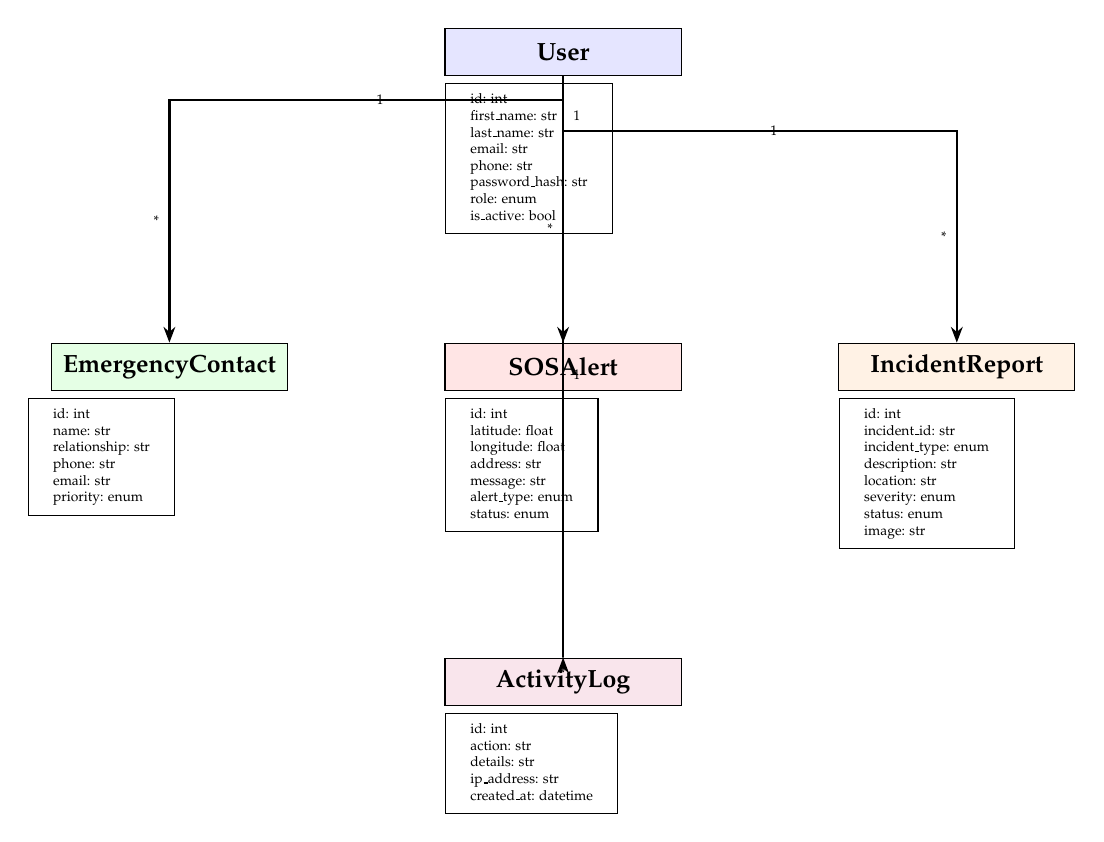
\begin{tikzpicture}[
    classbox/.style={rectangle, draw, minimum width=3cm, minimum height=0.6cm, text centered, font=\small},
    relation/.style={-{Stealth[length=2mm]}, thick},
  ]

    % User
    \node[classbox, fill=blue!10] (user) at (0, 3) {\textbf{User}};
    \node[rectangle, draw, anchor=north west, inner sep=3pt, font=\tiny] (userattrs) at (-1.5, 2.6) {
      \begin{tabular}{l}
        id: int \\
        first\_name: str \\
        last\_name: str \\
        email: str \\
        phone: str \\
        password\_hash: str \\
        role: enum \\
        is\_active: bool
      \end{tabular}
    };

    % EmergencyContact
    \node[classbox, fill=green!10] (contact) at (-5, -1) {\textbf{EmergencyContact}};
    \node[rectangle, draw, anchor=north west, inner sep=3pt, font=\tiny] (conattrs) at (-6.8, -1.4) {
      \begin{tabular}{l}
        id: int \\
        name: str \\
        relationship: str \\
        phone: str \\
        email: str \\
        priority: enum
      \end{tabular}
    };

    % SOSAlert
    \node[classbox, fill=red!10] (sos) at (0, -1) {\textbf{SOSAlert}};
    \node[rectangle, draw, anchor=north west, inner sep=3pt, font=\tiny] (sosattrs) at (-1.5, -1.4) {
      \begin{tabular}{l}
        id: int \\
        latitude: float \\
        longitude: float \\
        address: str \\
        message: str \\
        alert\_type: enum \\
        status: enum
      \end{tabular}
    };

    % IncidentReport
    \node[classbox, fill=orange!10] (incident) at (5, -1) {\textbf{IncidentReport}};
    \node[rectangle, draw, anchor=north west, inner sep=3pt, font=\tiny] (incattrs) at (3.5, -1.4) {
      \begin{tabular}{l}
        id: int \\
        incident\_id: str \\
        incident\_type: enum \\
        description: str \\
        location: str \\
        severity: enum \\
        status: enum \\
        image: str
      \end{tabular}
    };

    % ActivityLog
    \node[classbox, fill=purple!10] (activity) at (0, -5) {\textbf{ActivityLog}};
    \node[rectangle, draw, anchor=north west, inner sep=3pt, font=\tiny] (actattrs) at (-1.5, -5.4) {
      \begin{tabular}{l}
        id: int \\
        action: str \\
        details: str \\
        ip\_address: str \\
        created\_at: datetime
      \end{tabular}
    };

    % Relationships
    \draw[relation] (user.south) -- ++(0,-0.3) -| node[near start, right, font=\tiny] {1} node[near end, left, font=\tiny] {*} (contact.north);
    \draw[relation] (user.south) -- ++(0,-0.5) -| node[near start, right, font=\tiny] {1} node[near end, left, font=\tiny] {*} (sos.north);
    \draw[relation] (user.south) -- ++(0,-0.7) -| node[near start, right, font=\tiny] {1} node[near end, left, font=\tiny] {*} (incident.north);
    \draw[relation] (user.south) -- ++(0,-0.2) |- node[near start, right, font=\tiny] {1} node[near end, below, font=\tiny] {*} (activity.north);

  \end{tikzpicture}
  \caption{Class Diagram: Data Model and Relationships}
  \label{fig:class-diagram}
\end{figure}

\section{Module Description}

The SafeGuard system is organized into the following functional modules:

\subsection{Module 1: Authentication and User Management}

This module handles all aspects of user identity management, including registration, login, profile editing, password changes, and profile picture uploads. It implements JWT-based stateless authentication with 24-hour token expiry. The backend routes are defined in \texttt{app/api/auth.py} and \texttt{app/api/profile.py}, while the frontend state is managed through \texttt{AuthContext.jsx}.

\subsection{Module 2: Emergency Contact Management}

This module provides full CRUD functionality for emergency contacts, supporting name, relationship, phone number, email, and priority classification. Contacts can be searched across multiple fields and filtered by priority level. The UI presents contacts in a card-based layout with avatar initials and colour-coded priority indicators.

\subsection{Module 3: SOS Emergency Alert System}

The SOS module is the core safety feature, providing a prominent one-press button that triggers emergency alerts. Upon confirmation, the system captures geolocation coordinates using the browser's Geolocation API, associates them with the alert, and records the event. Alerts are classified by type (manual, automatic, panic, medical, fire, security) and tracked through status states (active, acknowledged, resolved, cancelled).

\subsection{Module 4: Incident Reporting and Tracking}

This module enables structured incident documentation with eight predefined incident types. Each report generates a unique identifier (INC-XXXXXXXX format) and captures description, location, coordinates, severity, and optional image evidence. Incidents progress through a lifecycle of pending, investigating, resolved, and closed statuses.

\subsection{Module 5: History and Analytics}

This module combines SOS alert history and incident history into a tabbed view with pagination, multi-criteria filtering, and search. It includes CSV export functionality for offline record-keeping. The dashboard aggregates real-time statistics including total contacts, total alerts, active alerts, and total incidents.

\subsection{Module 6: Activity Logging}

A cross-cutting concern implemented across all modules, this system records every significant user action (registration, login, SOS trigger, incident report, profile update, password change) in the activity\_logs table with action type, descriptive details, IP address, and timestamp.


% Chapter 4: Database Design
% ============================================================
% CHAPTER 4: DATABASE DESIGN
% ============================================================
\chapter{Database Design}

This chapter presents the database design for the SafeGuard system, including the database overview, Entity-Relationship modelling, detailed schema definitions, table structures with their attributes, key constraints, relationships, and a comprehensive data dictionary.

\section{Database Overview}

The SafeGuard system uses \textbf{MySQL 8.0} as its relational database management system (RDBMS). MySQL was selected for its reliability, performance, widespread adoption in web applications, and excellent compatibility with Python's SQLAlchemy ORM through the PyMySQL driver.

The database, named \texttt{safety\_alert\_db}, is managed through SQLAlchemy's declarative base system, which maps Python classes to database tables. The schema is automatically created at application startup using \texttt{Base.metadata.create\_all()}, eliminating the need for manual SQL migration scripts during development.

The database follows the \textbf{Third Normal Form (3NF)} of normalization, ensuring minimal data redundancy and optimal data integrity. The schema comprises five primary tables, each representing a distinct entity in the system's domain model.

\begin{table}[H]
  \centering
  \caption{Database Tables Overview}
  \label{tab:db-overview}
  \begin{tabularx}{\textwidth}{@{}l X c@{}}
    \toprule
    \textbf{Table Name} & \textbf{Purpose} & \textbf{Est. Records} \\
    \midrule
    \texttt{users} & Stores user account information, credentials, and profile data & 1--1000 \\
    \texttt{emergency\_contacts} & Stores user-managed emergency contact details & 1--50 per user \\
    \texttt{sos\_alerts} & Records all SOS emergency alert events & 0--100 per user \\
    \texttt{incident\_reports} & Stores structured incident reports with status tracking & 0--50 per user \\
    \texttt{activity\_logs} & Logs all significant user actions for audit purposes & 5--200 per user \\
    \bottomrule
  \end{tabularx}
\end{table}

\section{Entity-Relationship Diagram}

Figure~\ref{fig:er-diagram} presents the Entity-Relationship (ER) diagram for the SafeGuard database, illustrating the entities, attributes, and relationships between tables.

\begin{figure}[H]
  \centering
  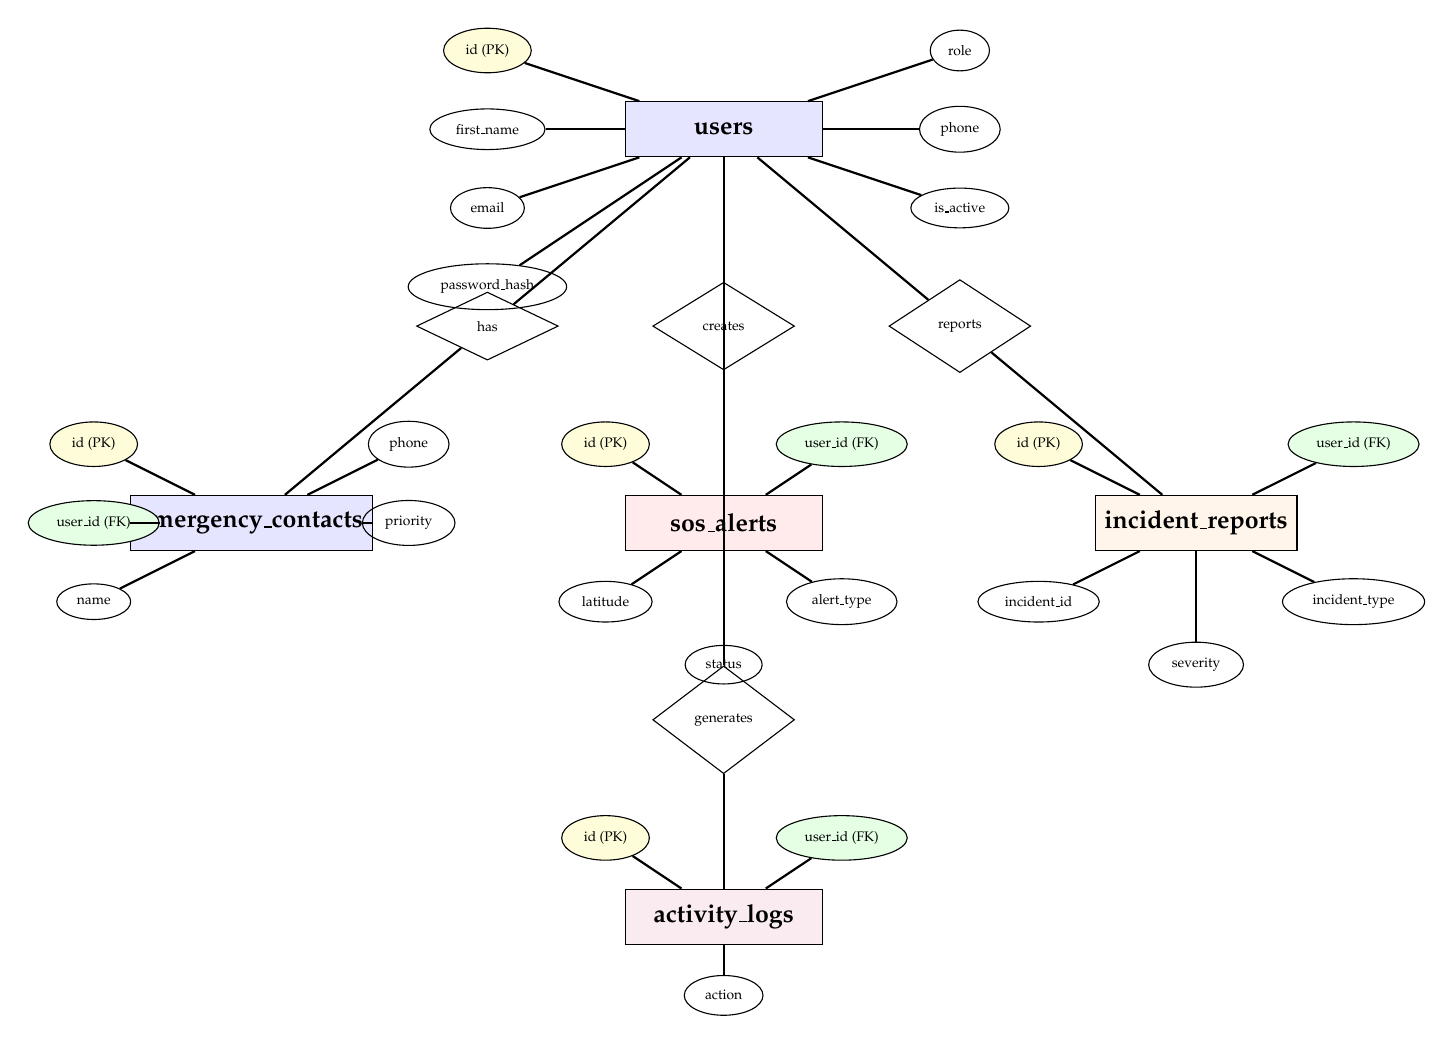
\begin{tikzpicture}[
    entity/.style={rectangle, draw, minimum width=2.5cm, minimum height=0.7cm, text centered, font=\small\bfseries, fill=blue!10},
    weakentity/.style={rectangle, draw, dashed, minimum width=2.5cm, minimum height=0.7cm, text centered, font=\small\bfseries, fill=red!5},
    relation/.style={diamond, draw, minimum width=1.8cm, minimum height=0.6cm, text centered, font=\tiny},
    pkattr/.style={ellipse, draw, fill=yellow!15, font=\tiny},
    fkattr/.style={ellipse, draw, fill=green!10, font=\tiny},
    normattr/.style={ellipse, draw, font=\tiny},
    line/.style={thick},
  ]

    % User Entity
    \node[entity] (user) at (0, 0) {users};
    \node[pkattr] (uid) at (-3, 1) {id (PK)};
    \node[normattr] (uname) at (-3, 0) {first\_name};
    \node[normattr] (uemail) at (-3, -1) {email};
    \node[normattr] (upass) at (-3, -2) {password\_hash};
    \node[normattr] (urole) at (3, 1) {role};
    \node[normattr] (uphone) at (3, 0) {phone};
    \node[normattr] (uactive) at (3, -1) {is\_active};
    \draw[line] (user) -- (uid);
    \draw[line] (user) -- (uname);
    \draw[line] (user) -- (uemail);
    \draw[line] (user) -- (upass);
    \draw[line] (user) -- (urole);
    \draw[line] (user) -- (uphone);
    \draw[line] (user) -- (uactive);

    % Emergency Contact Entity
    \node[entity] (contact) at (-6, -5) {emergency\_contacts};
    \node[pkattr] (cid) at (-8, -4) {id (PK)};
    \node[fkattr] (cuid) at (-8, -5) {user\_id (FK)};
    \node[normattr] (cname) at (-8, -6) {name};
    \node[normattr] (cphone) at (-4, -4) {phone};
    \node[normattr] (cpriority) at (-4, -5) {priority};
    \draw[line] (contact) -- (cid);
    \draw[line] (contact) -- (cuid);
    \draw[line] (contact) -- (cname);
    \draw[line] (contact) -- (cphone);
    \draw[line] (contact) -- (cpriority);

    % SOS Alert Entity
    \node[entity, fill=red!8] (sos) at (0, -5) {sos\_alerts};
    \node[pkattr] (sid) at (-1.5, -4) {id (PK)};
    \node[fkattr] (suid) at (1.5, -4) {user\_id (FK)};
    \node[normattr] (slat) at (-1.5, -6) {latitude};
    \node[normattr] (stype) at (1.5, -6) {alert\_type};
    \node[normattr] (sstatus) at (0, -6.8) {status};
    \draw[line] (sos) -- (sid);
    \draw[line] (sos) -- (suid);
    \draw[line] (sos) -- (slat);
    \draw[line] (sos) -- (stype);
    \draw[line] (sos) -- (sstatus);

    % Incident Entity
    \node[entity, fill=orange!8] (incident) at (6, -5) {incident\_reports};
    \node[pkattr] (iid) at (4, -4) {id (PK)};
    \node[fkattr] (iuid) at (8, -4) {user\_id (FK)};
    \node[normattr] (iincid) at (4, -6) {incident\_id};
    \node[normattr] (itype) at (8, -6) {incident\_type};
    \node[normattr] (isev) at (6, -6.8) {severity};
    \draw[line] (incident) -- (iid);
    \draw[line] (incident) -- (iuid);
    \draw[line] (incident) -- (iincid);
    \draw[line] (incident) -- (itype);
    \draw[line] (incident) -- (isev);

    % Activity Log Entity
    \node[entity, fill=purple!8] (activity) at (0, -10) {activity\_logs};
    \node[pkattr] (aid) at (-1.5, -9) {id (PK)};
    \node[fkattr] (auid) at (1.5, -9) {user\_id (FK)};
    \node[normattr] (aaction) at (0, -11) {action};
    \draw[line] (activity) -- (aid);
    \draw[line] (activity) -- (auid);
    \draw[line] (activity) -- (aaction);

    % Relations
    \node[relation] (r1) at (-3, -2.5) {has};
    \node[relation] (r2) at (0, -2.5) {creates};
    \node[relation] (r3) at (3, -2.5) {reports};
    \node[relation] (r4) at (0, -7.5) {generates};

    \draw[line] (user) -- (r1);
    \draw[line] (r1) -- (contact);
    \draw[line] (user) -- (r2);
    \draw[line] (r2) -- (sos);
    \draw[line] (user) -- (r3);
    \draw[line] (r3) -- (incident);
    \draw[line] (user) -- (r4);
    \draw[line] (r4) -- (activity);

  \end{tikzpicture}
  \caption{Entity-Relationship Diagram}
  \label{fig:er-diagram}
\end{figure}

\section{Database Schema}

The SafeGuard database schema is defined through SQLAlchemy ORM model classes. Each model class maps to a corresponding database table with columns, constraints, and relationships defined at the class level. The ORM approach ensures database portability and type-safe data access.

\section{Table Definitions}

\subsection{Users Table}

The \texttt{users} table is the central entity storing user account information and authentication credentials.

\begin{table}[H]
  \centering
  \caption{Users Table Schema}
  \label{tab:schema-users}
  \begin{tabularx}{\textwidth}{@{}l l l X l@{}}
    \toprule
    \textbf{Column} & \textbf{Type} & \textbf{Constraints} & \textbf{Description} & \textbf{Default} \\
    \midrule
    id & INTEGER & PK, AUTO\_INCREMENT & Unique user identifier & --- \\
    first\_name & VARCHAR(100) & NOT NULL & User's first name & --- \\
    last\_name & VARCHAR(100) & NOT NULL & User's last name & --- \\
    email & VARCHAR(255) & UNIQUE, NOT NULL, INDEX & User's email address & --- \\
    phone & VARCHAR(20) & NOT NULL & Contact phone number & --- \\
    password\_hash & VARCHAR(255) & NOT NULL & bcrypt hashed password & --- \\
    profile\_picture & VARCHAR(500) & NULLABLE & Path to profile image & NULL \\
    role & ENUM & NOT NULL & User or admin role & 'user' \\
    is\_active & BOOLEAN & NOT NULL & Account active status & TRUE \\
    created\_at & TIMESTAMP & NOT NULL & Account creation time & NOW() \\
    updated\_at & TIMESTAMP & NOT NULL & Last update timestamp & NOW() \\
    \bottomrule
  \end{tabularx}
\end{table}

\subsection{Emergency Contacts Table}

The \texttt{emergency\_contacts} table stores the emergency contact details for each user.

\begin{table}[H]
  \centering
  \caption{Emergency Contacts Table Schema}
  \label{tab:schema-contacts}
  \begin{tabularx}{\textwidth}{@{}l l l X l@{}}
    \toprule
    \textbf{Column} & \textbf{Type} & \textbf{Constraints} & \textbf{Description} & \textbf{Default} \\
    \midrule
    id & INTEGER & PK, AUTO\_INCREMENT & Unique contact identifier & --- \\
    user\_id & INTEGER & FK $\to$ users.id, NOT NULL, INDEX & Owner user reference & --- \\
    name & VARCHAR(200) & NOT NULL & Contact person's name & --- \\
    relationship & VARCHAR(100) & NOT NULL & Relationship type & --- \\
    phone & VARCHAR(20) & NOT NULL & Contact phone number & --- \\
    email & VARCHAR(255) & NULLABLE & Contact email address & NULL \\
    priority & ENUM & NOT NULL & Priority level & 'medium' \\
    created\_at & TIMESTAMP & NOT NULL & Creation timestamp & NOW() \\
    updated\_at & TIMESTAMP & NOT NULL & Last update timestamp & NOW() \\
    \bottomrule
  \end{tabularx}
\end{table}

\subsection{SOS Alerts Table}

The \texttt{sos\_alerts} table records all emergency alert events triggered by users.

\begin{table}[H]
  \centering
  \caption{SOS Alerts Table Schema}
  \label{tab:schema-sos}
  \begin{tabularx}{\textwidth}{@{}l l l X l@{}}
    \toprule
    \textbf{Column} & \textbf{Type} & \textbf{Constraints} & \textbf{Description} & \textbf{Default} \\
    \midrule
    id & INTEGER & PK, AUTO\_INCREMENT & Unique alert identifier & --- \\
    user\_id & INTEGER & FK $\to$ users.id, NOT NULL, INDEX & Alert creator reference & --- \\
    latitude & NUMERIC(10,8) & NULLABLE & GPS latitude coordinate & NULL \\
    longitude & NUMERIC(11,8) & NULLABLE & GPS longitude coordinate & NULL \\
    address & TEXT & NULLABLE & Textual location description & NULL \\
    message & TEXT & NULLABLE & Custom emergency message & NULL \\
    alert\_type & ENUM & NOT NULL & Alert classification & 'manual' \\
    status & ENUM & NOT NULL, INDEX & Alert lifecycle status & 'active' \\
    created\_at & TIMESTAMP & NOT NULL & Alert creation time & NOW() \\
    updated\_at & TIMESTAMP & NOT NULL & Last status update & NOW() \\
    \bottomrule
  \end{tabularx}
\end{table}

\subsection{Incident Reports Table}

The \texttt{incident\_reports} table stores structured safety incident reports.

\begin{table}[H]
  \centering
  \caption{Incident Reports Table Schema}
  \label{tab:schema-incident}
  \begin{tabularx}{\textwidth}{@{}l l l X l@{}}
    \toprule
    \textbf{Column} & \textbf{Type} & \textbf{Constraints} & \textbf{Description} & \textbf{Default} \\
    \midrule
    id & INTEGER & PK, AUTO\_INCREMENT & Internal record ID & --- \\
    user\_id & INTEGER & FK $\to$ users.id, NOT NULL, INDEX & Report creator reference & --- \\
    incident\_id & VARCHAR(50) & UNIQUE, NOT NULL, INDEX & Public incident ID (INC-XXXXXXXX) & --- \\
    incident\_type & ENUM & NOT NULL & Type of incident & --- \\
    description & TEXT & NOT NULL & Detailed incident description & --- \\
    location & VARCHAR(500) & NOT NULL & Location text & --- \\
    latitude & NUMERIC(10,8) & NULLABLE & GPS latitude & NULL \\
    longitude & NUMERIC(11,8) & NULLABLE & GPS longitude & NULL \\
    severity & ENUM & NOT NULL & Severity level & 'medium' \\
    image & VARCHAR(500) & NULLABLE & Evidence image path & NULL \\
    status & ENUM & NOT NULL & Investigation status & 'pending' \\
    created\_at & TIMESTAMP & NOT NULL & Report creation time & NOW() \\
    updated\_at & TIMESTAMP & NOT NULL & Last update timestamp & NOW() \\
    \bottomrule
  \end{tabularx}
\end{table}

\subsection{Activity Logs Table}

The \texttt{activity\_logs} table provides an audit trail of all significant user actions.

\begin{table}[H]
  \centering
  \caption{Activity Logs Table Schema}
  \label{tab:schema-activity}
  \begin{tabularx}{\textwidth}{@{}l l l X l@{}}
    \toprule
    \textbf{Column} & \textbf{Type} & \textbf{Constraints} & \textbf{Description} & \textbf{Default} \\
    \midrule
    id & INTEGER & PK, AUTO\_INCREMENT & Unique log entry ID & --- \\
    user\_id & INTEGER & FK $\to$ users.id, NOT NULL, INDEX & Action performer reference & --- \\
    action & VARCHAR(100) & NOT NULL & Action type identifier & --- \\
    details & TEXT & NULLABLE & Descriptive action details & NULL \\
    ip\_address & VARCHAR(45) & NULLABLE & Client IP address & NULL \\
    created\_at & TIMESTAMP & NOT NULL & Action timestamp & NOW() \\
    \bottomrule
  \end{tabularx}
\end{table}

\section{Relationships}

The SafeGuard database employs the following relationships:

\begin{table}[H]
  \centering
  \caption{Database Relationships}
  \label{tab:relationships}
  \begin{tabularx}{\textwidth}{@{}l l l X@{}}
    \toprule
    \textbf{Parent Table} & \textbf{Child Table} & \textbf{Type} & \textbf{Description} \\
    \midrule
    users & emergency\_contacts & One-to-Many & A user can have many emergency contacts; each contact belongs to one user. Cascade delete ensures contacts are removed when a user is deleted. \\
    users & sos\_alerts & One-to-Many & A user can trigger many SOS alerts; each alert is associated with one user. Cascade delete ensures alerts are removed with the user. \\
    users & incident\_reports & One-to-Many & A user can file many incident reports; each report belongs to one user. Cascade delete ensures reports are removed with the user. \\
    users & activity\_logs & One-to-Many & A user generates many activity log entries; each entry is associated with one user. Cascade delete ensures logs are removed with the user. \\
    \bottomrule
  \end{tabularx}
\end{table}

All foreign key constraints use \texttt{ON DELETE CASCADE}, ensuring referential integrity is maintained when parent records are removed. This design simplifies data management while ensuring no orphaned records exist in child tables.

\section{Primary and Foreign Keys}

\begin{itemize}
  \item \textbf{Primary Keys:} All tables use auto-incrementing integer primary keys (\texttt{id}), except the \texttt{incident\_id} field in \texttt{incident\_reports} which serves as a secondary unique key with the format \texttt{INC-XXXXXXXX}.

  \item \textbf{Foreign Keys:} The \texttt{user\_id} column in \texttt{emergency\_contacts}, \texttt{sos\_alerts}, \texttt{incident\_reports}, and \texttt{activity\_logs} tables references the \texttt{id} column in the \texttt{users} table, establishing the owner relationship.

  \item \textbf{Indexes:} Indexes are created on all foreign key columns for query optimization, as well as on frequently queried columns including \texttt{email} (users), \texttt{incident\_id} (incident\_reports), and \texttt{status} (sos\_alerts).
\end{itemize}

\section{Data Dictionary}

\begin{table}[H]
  \centering
  \caption{Data Dictionary: ENUM Types}
  \label{tab:data-dict}
  \begin{tabularx}{\textwidth}{@{}l l X@{}}
    \toprule
    \textbf{ENUM Field} & \textbf{Values} & \textbf{Description} \\
    \midrule
    user.role & user, admin & System role: standard user or administrator \\
    emergency\_contacts.priority & low, medium, high, critical & Contact priority for emergency notification \\
    sos\_alerts.alert\_type & manual, automatic, panic, medical, fire, security & Classification of the emergency \\
    sos\_alerts.status & active, acknowledged, resolved, cancelled & Alert lifecycle state \\
    incident\_reports.incident\_type & theft, assault, accident, fire, harassment, vandalism, medical, other & Nature of the reported incident \\
    incident\_reports.severity & low, medium, high, critical & Impact level of the incident \\
    incident\_reports.status & pending, investigating, resolved, closed & Investigation progress state \\
    \bottomrule
  \end{tabularx}
\end{table}

\begin{table}[H]
  \centering
  \caption{Data Dictionary: Data Types}
  \label{tab:data-types}
  \begin{tabularx}{\textwidth}{@{}l l X@{}}
    \toprule
    \textbf{Data Type} & \textbf{SQL Equivalent} & \textbf{Usage} \\
    \midrule
    VARCHAR(n) & VARCHAR(n) & Variable-length string with specified maximum length \\
    TEXT & TEXT & Variable-length string for long content (descriptions, addresses) \\
    INTEGER & INT & Whole numbers (IDs, counts) \\
    BOOLEAN & TINYINT(1) / BIT & True/false values \\
    NUMERIC(10,8) & DECIMAL(10,8) & GPS coordinates with 8 decimal places of precision \\
    TIMESTAMP & DATETIME & Date and time values \\
    ENUM & ENUM & Predefined set of allowed values \\
    \bottomrule
  \end{tabularx}
\end{table}

\section{Sample Data}

This section presents sample data stored in each database table to illustrate the actual data patterns and relationships in the SafeGuard system.

\subsection{Users Table Data}

Figure~\ref{fig:data-users} shows sample records from the \texttt{users} table, demonstrating user account information including credentials, profile data, and role assignments.

\begin{figure}[H]
  \centering
  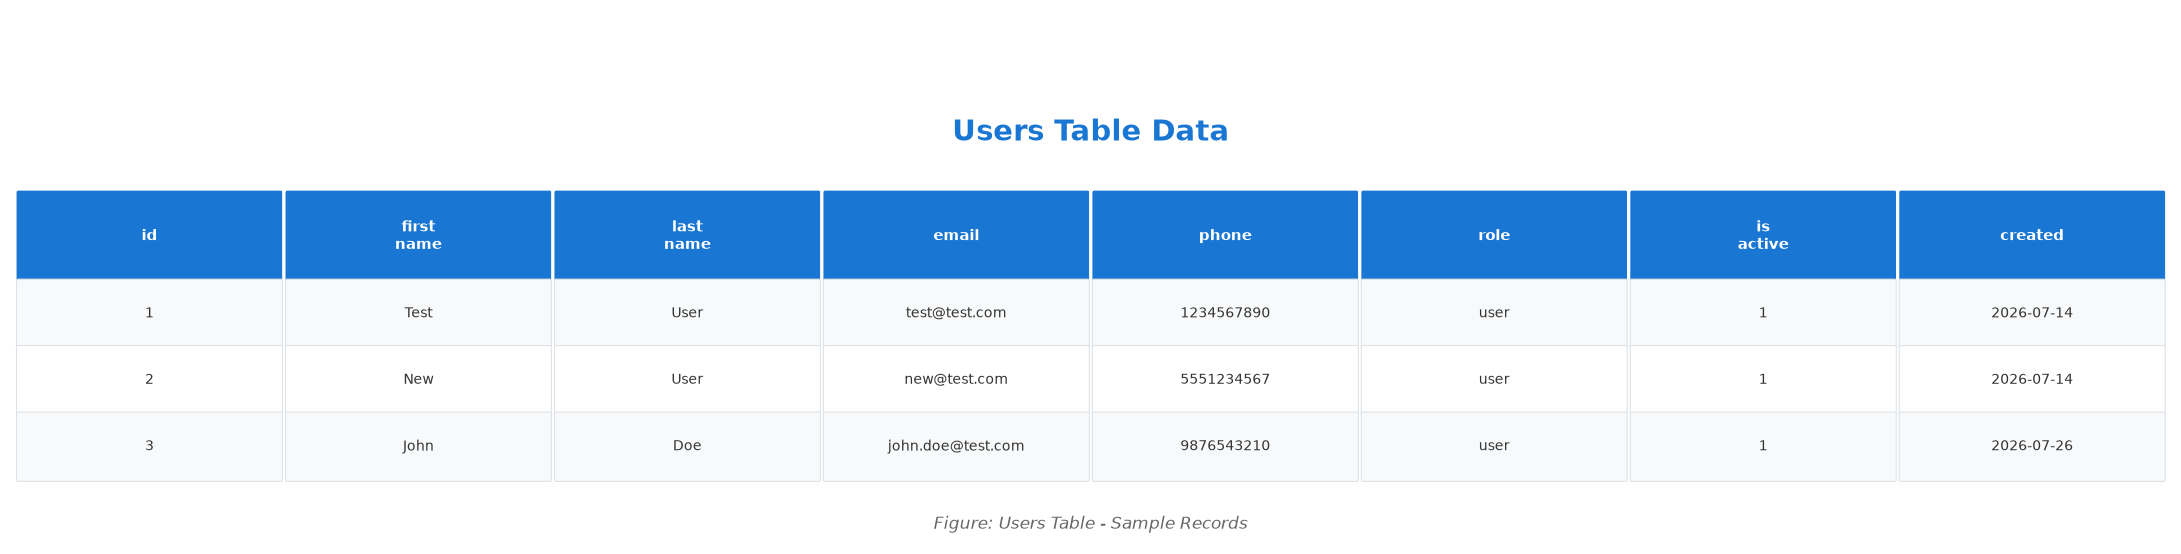
\includegraphics[width=0.95\textwidth]{db_users.png}
  \caption{Sample Data: Users Table}
  \label{fig:data-users}
\end{figure}

\subsection{Emergency Contacts Table Data}

Figure~\ref{fig:data-contacts} shows sample emergency contact records with priority classifications.

\begin{figure}[H]
  \centering
  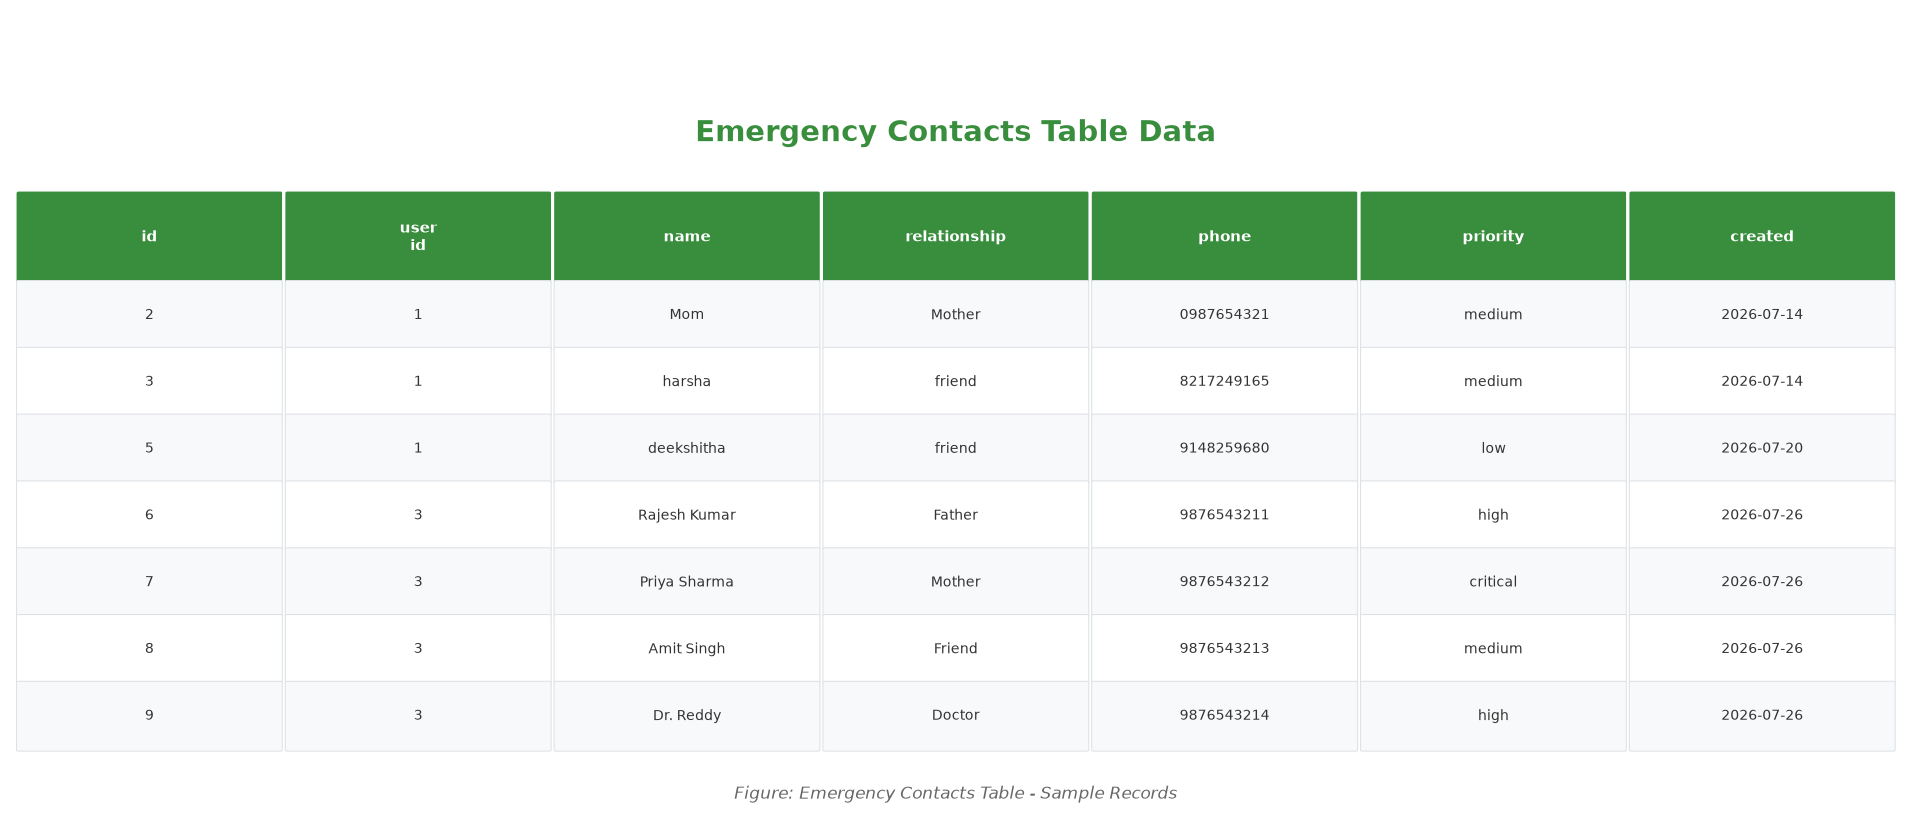
\includegraphics[width=0.95\textwidth]{db_emergency_contacts.png}
  \caption{Sample Data: Emergency Contacts Table}
  \label{fig:data-contacts}
\end{figure}

\subsection{SOS Alerts Table Data}

Figure~\ref{fig:data-sos} shows sample SOS alert records with geolocation and status tracking.

\begin{figure}[H]
  \centering
  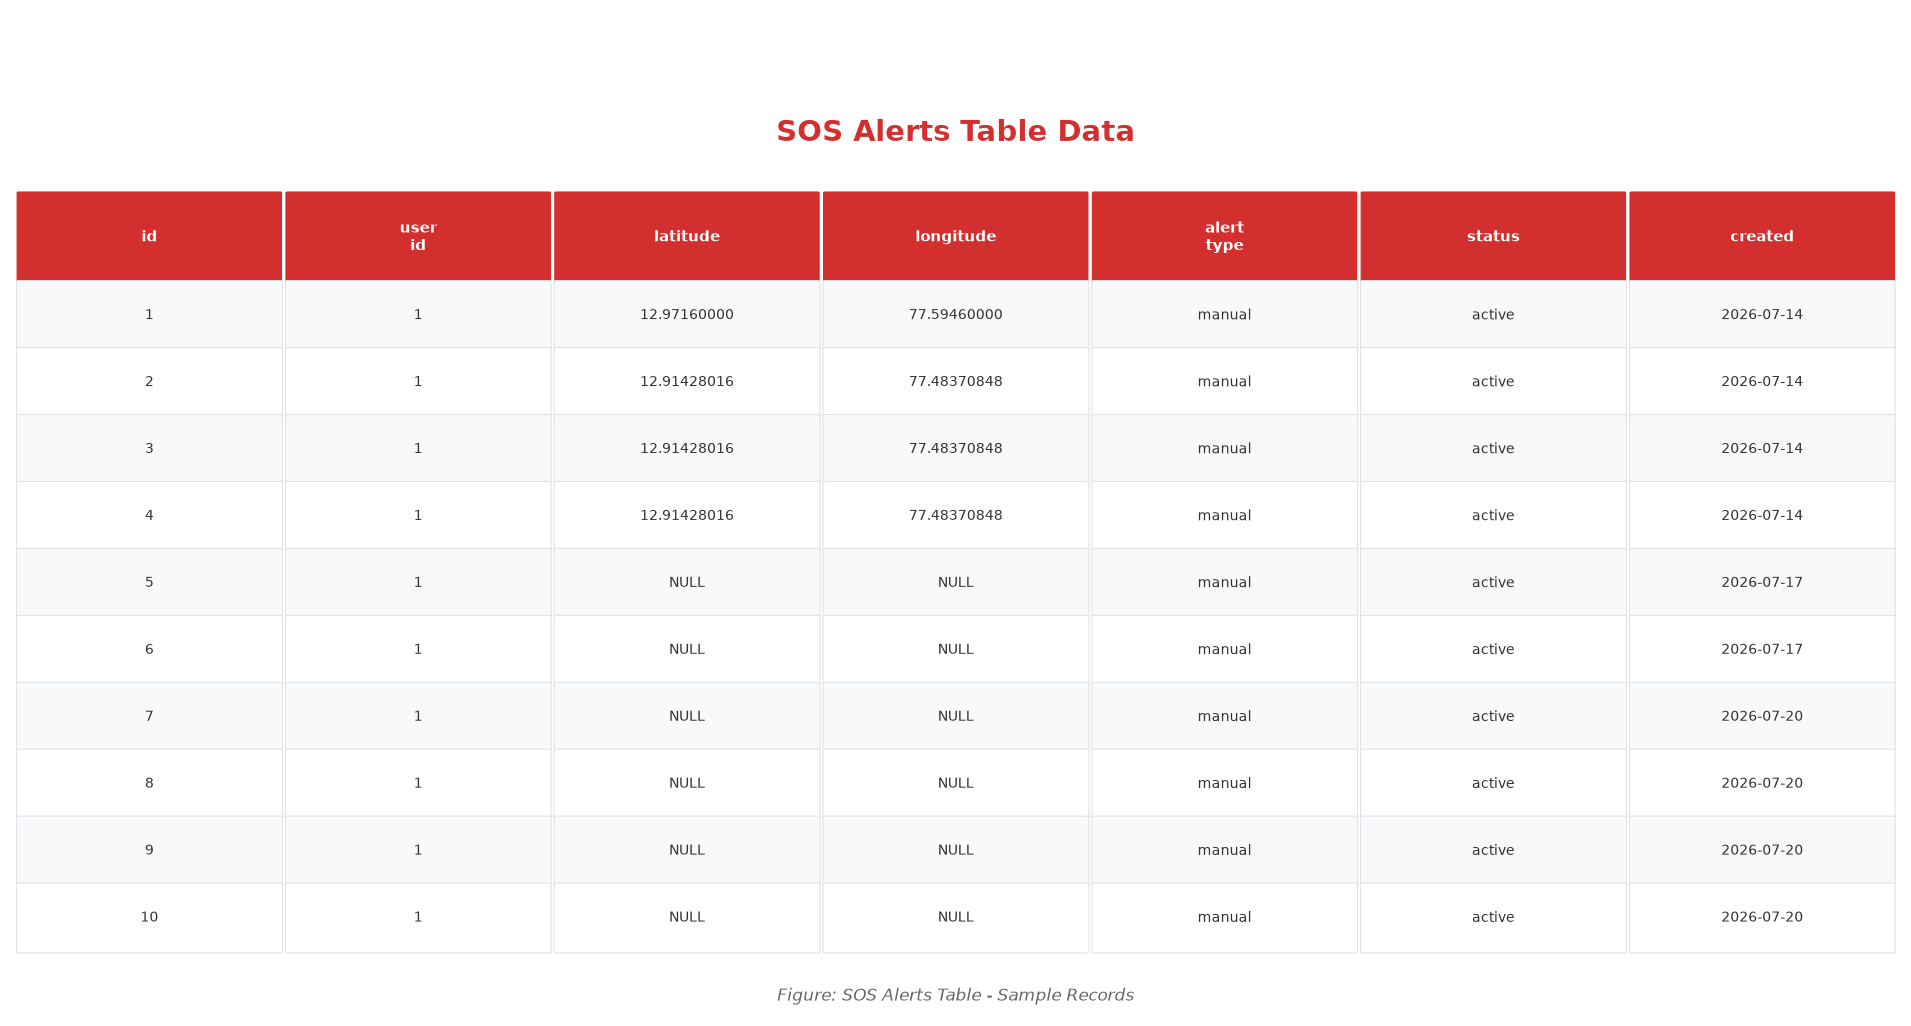
\includegraphics[width=0.95\textwidth]{db_sos_alerts.png}
  \caption{Sample Data: SOS Alerts Table}
  \label{fig:data-sos}
\end{figure}

\subsection{Incident Reports Table Data}

Figure~\ref{fig:data-incidents} shows sample incident reports with type, severity, and status tracking.

\begin{figure}[H]
  \centering
  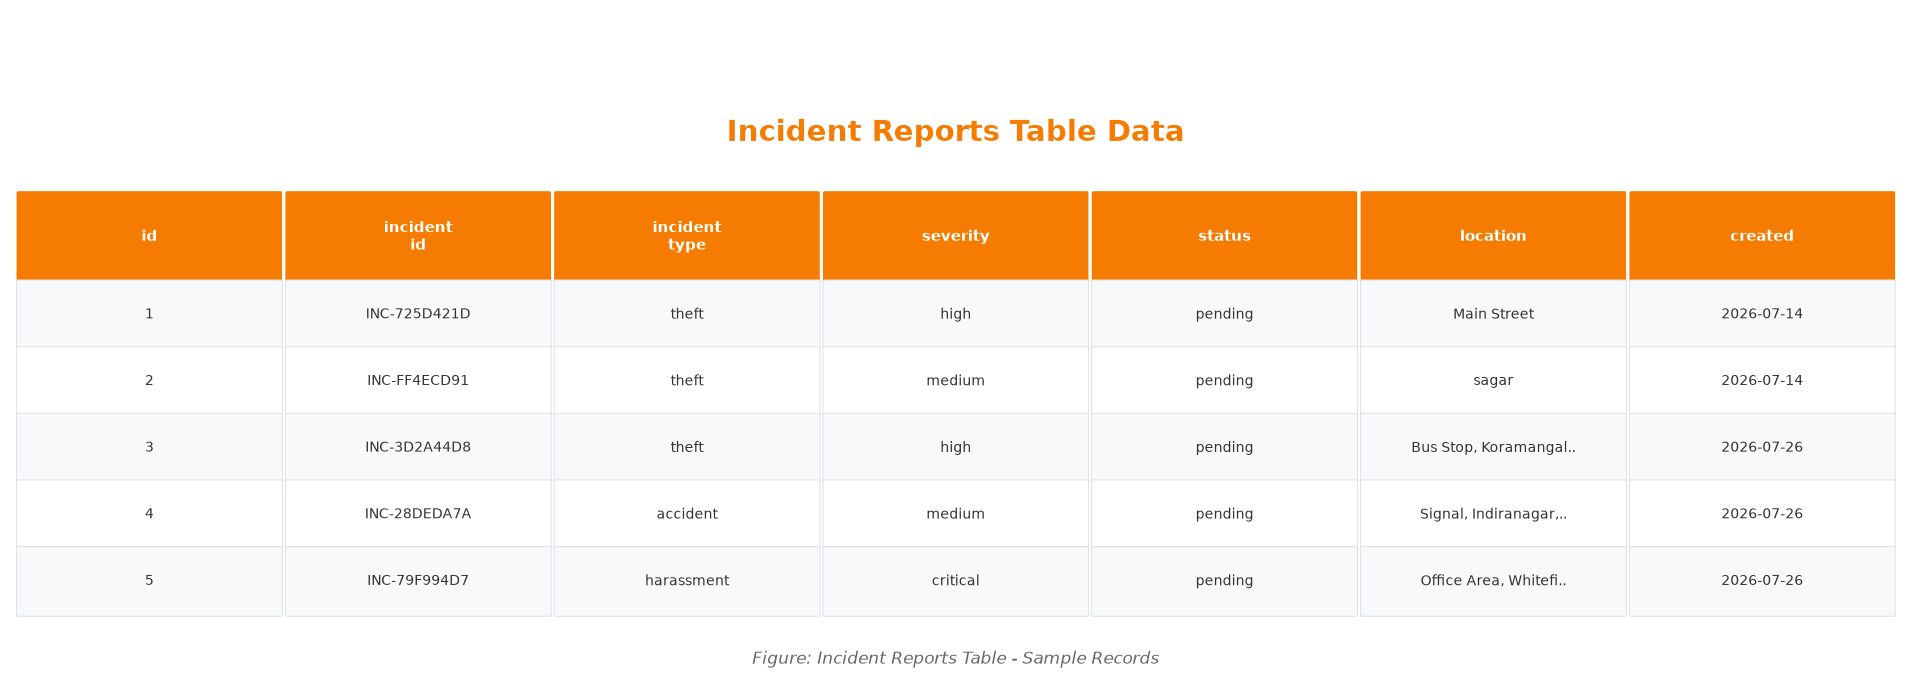
\includegraphics[width=0.95\textwidth]{db_incident_reports.png}
  \caption{Sample Data: Incident Reports Table}
  \label{fig:data-incidents}
\end{figure}

\subsection{Activity Logs Table Data}

Figure~\ref{fig:data-activity} shows sample activity log entries tracking user actions.

\begin{figure}[H]
  \centering
  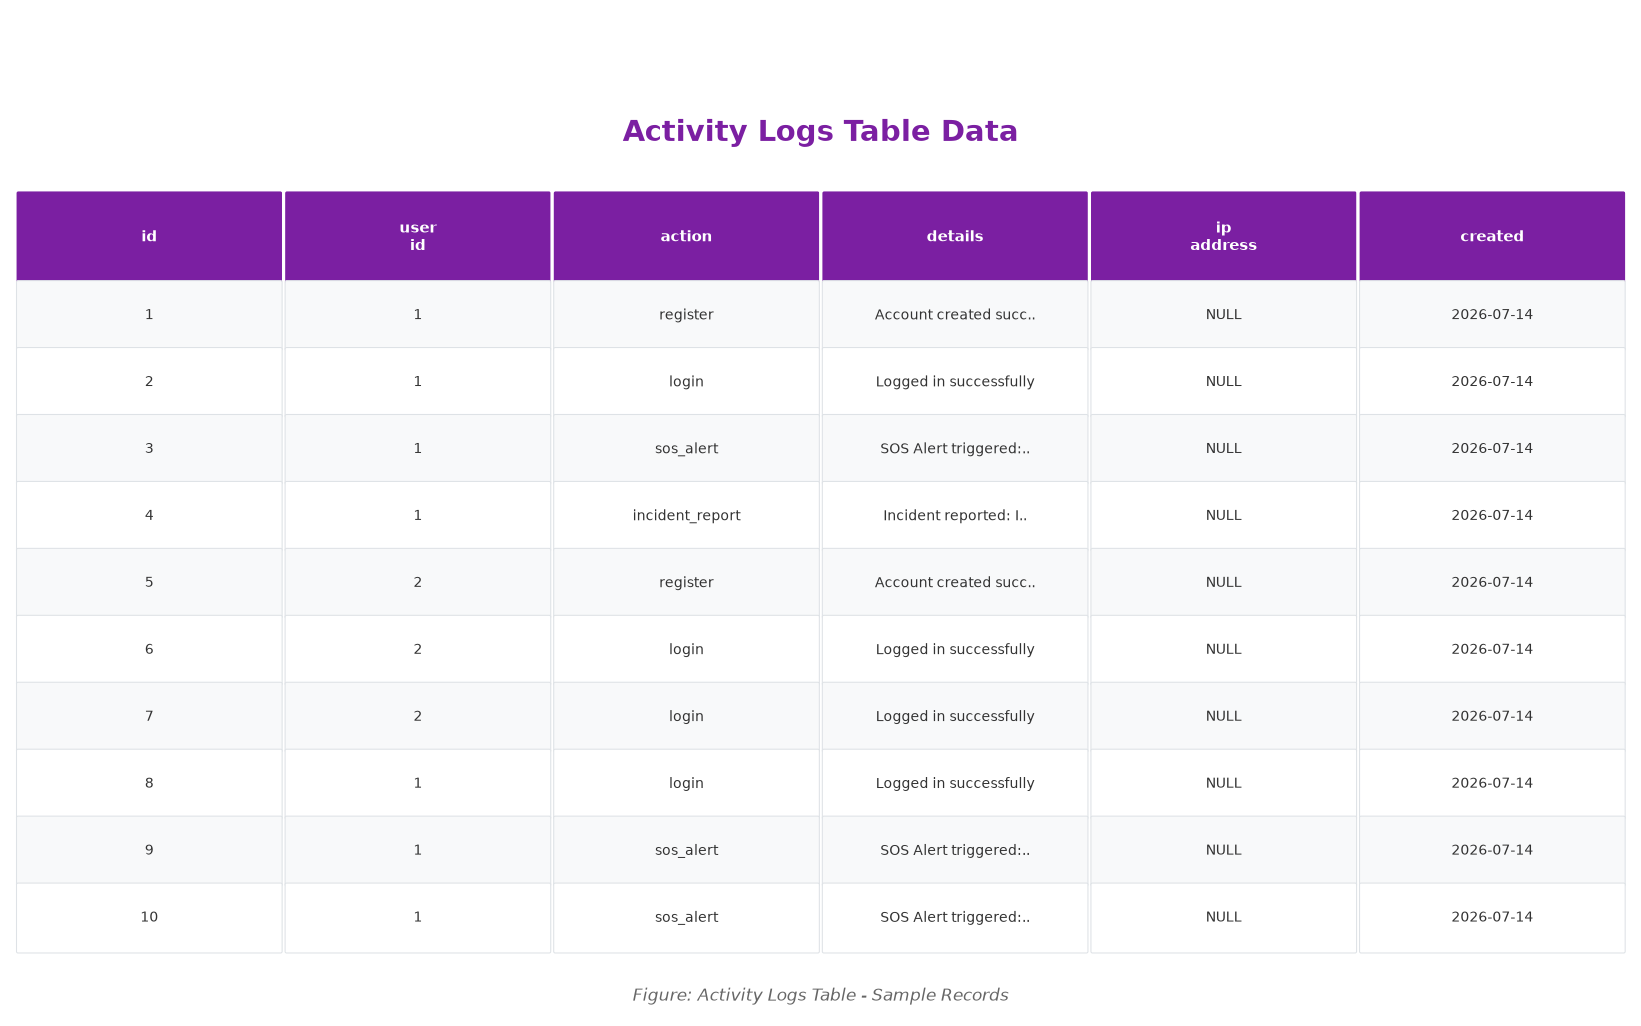
\includegraphics[width=0.95\textwidth]{db_activity_logs.png}
  \caption{Sample Data: Activity Logs Table}
  \label{fig:data-activity}
\end{figure}


% Chapter 5: Implementation
% ============================================================
% CHAPTER 5: IMPLEMENTATION
% ============================================================
\chapter{Implementation}

This chapter provides a detailed account of the implementation of the SafeGuard system. It covers the technologies and tools employed, hardware and software requirements, project module implementations, key algorithms and workflows, code structure, and specific implementation details for each functional module.

\section{Technologies Used}

The SafeGuard system employs a modern technology stack chosen for their maturity, community support, performance characteristics, and suitability for the project's requirements.

\subsection{Backend Technologies}

\begin{table}[H]
  \centering
  \caption{Backend Technology Stack}
  \label{tab:tech-backend}
  \begin{tabularx}{\textwidth}{@{}l l X@{}}
    \toprule
    \textbf{Technology} & \textbf{Version} & \textbf{Purpose} \\
    \midrule
    Python & 3.9+ & Primary programming language for backend development \\
    FastAPI & $\geq$0.115.0 & High-performance asynchronous web framework for RESTful API development \\
    Uvicorn & $\geq$0.32.0 & ASGI server for serving the FastAPI application \\
    SQLAlchemy & $\geq$2.0.36 & Object-Relational Mapping (ORM) library for database interaction \\
    PyMySQL & $\geq$1.1.0 & Pure-Python MySQL database driver \\
    Pydantic & $\geq$2.10.0 & Data validation and settings management using Python type annotations \\
    bcrypt & $\geq$4.2.0 & Password hashing library with salt generation \\
    python-jose & $\geq$3.3.0 & JSON Object Signing and Encryption (JOSE) library for JWT handling \\
    python-dotenv & $\geq$1.0.0 & Environment variable management from .env files \\
    aiofiles & $\geq$24.1.0 & Asynchronous file operations for profile picture uploads \\
    python-multipart & $\geq$0.0.12 & Multipart form data parsing for file uploads \\
    cryptography & $\geq$44.0.0 & Cryptographic primitives for secure operations \\
    \bottomrule
  \end{tabularx}
\end{table}

\subsection{Frontend Technologies}

\begin{table}[H]
  \centering
  \caption{Frontend Technology Stack}
  \label{tab:tech-frontend}
  \begin{tabularx}{\textwidth}{@{}l l X@{}}
    \toprule
    \textbf{Technology} & \textbf{Version} & \textbf{Purpose} \\
    \midrule
    JavaScript (ES6+) & ES2022 & Primary programming language for frontend development \\
    React.js & 18.2.0 & Component-based UI library for building interactive interfaces \\
    React Router DOM & 6.21.1 & Declarative routing for single-page application navigation \\
    Material UI (MUI) & 5.15.1 & Comprehensive React component library implementing Material Design \\
    Emotion & $\geq$11.11.1 & CSS-in-JS styling library used by MUI \\
    Axios & 1.6.2 & Promise-based HTTP client for API communication \\
    react-hot-toast & 2.4.1 & Lightweight toast notification library \\
    Recharts & 2.10.3 & Composable charting library for dashboard visualizations \\
    Inter Font & 300--800 & Modern sans-serif typeface from Google Fonts \\
    \bottomrule
  \end{tabularx}
\end{table}

\subsection{Database}

\begin{table}[H]
  \centering
  \caption{Database Technology}
  \label{tab:tech-database}
  \begin{tabularx}{\textwidth}{@{}l X@{}}
    \toprule
    \textbf{Technology} & \textbf{Purpose} \\
    \midrule
    MySQL 8.0 & Relational database management system for persistent data storage \\
    SQLAlchemy ORM & Database abstraction layer providing Python-native data access \\
    PyMySQL & Database connectivity driver for Python-MySQL communication \\
    \bottomrule
  \end{tabularx}
\end{table}

\section{Software Requirements}

The following software is required to set up and run the SafeGuard system:

\begin{table}[H]
  \centering
  \caption{Software Requirements}
  \label{tab:software-req}
  \begin{tabularx}{\textwidth}{@{}l l X@{}}
    \toprule
    \textbf{Software} & \textbf{Version} & \textbf{Purpose} \\
    \midrule
    Python & 3.9 or higher & Backend runtime environment \\
    Node.js & 18.0 or higher & Frontend build and development server \\
    npm & 9.0 or higher & Frontend package management \\
    MySQL Server & 8.0 or higher & Database server \\
    Modern Web Browser & Latest & Application access (Chrome, Firefox, Safari, Edge) \\
    Code Editor & Latest & Development environment (VS Code recommended) \\
    \bottomrule
  \end{tabularx}
\end{table}

\section{Hardware Requirements}

\begin{table}[H]
  \centering
  \caption{Hardware Requirements for Development}
  \label{tab:hardware-req}
  \begin{tabularx}{\textwidth}{@{}l X@{}}
    \toprule
    \textbf{Component} & \textbf{Specification} \\
    \midrule
    Processor & Intel Core i5 or equivalent (minimum), Intel Core i7 or higher (recommended) \\
    Memory (RAM) & 8 GB minimum, 16 GB recommended \\
    Storage & 256 GB SSD minimum (for development tools and databases) \\
    Internet & Broadband connection for package installation and API testing \\
    Display & 1920 $\times$ 1080 resolution minimum for development \\
    \bottomrule
  \end{tabularx}
\end{table}

\section{Project Modules}

The SafeGuard system is organized into the following implementation modules, each representing a cohesive unit of functionality.

\subsection{Module 1: Authentication Module}

\textbf{Files:} \texttt{app/api/auth.py}, \texttt{app/auth/jwt.py}, \texttt{app/auth/dependencies.py}, \texttt{frontend/src/context/AuthContext.jsx}

The authentication module implements the complete user identity lifecycle. The backend exposes two endpoints: \texttt{POST /api/register} for new user creation and \texttt{POST /api/login} for existing user authentication.

The registration process validates input using Pydantic schemas, enforces email uniqueness, hashes passwords with bcrypt (12 rounds of salt generation), creates the user record, and issues a JWT token. The login process performs email lookup, bcrypt hash verification, activity logging, and JWT issuance.

The frontend manages authentication state through React Context (\texttt{AuthContext}), which stores the access token and user object in \texttt{localStorage}. Axios interceptors automatically attach the \texttt{Authorization: Bearer} header to outgoing requests and redirect to the login page upon receiving 401 responses.

\subsection{Module 2: Contact Management Module}

\textbf{Files:} \texttt{app/api/contacts.py}, \texttt{app/models/contact.py}, \texttt{app/schemas/contact.py}, \texttt{frontend/src/pages/Contacts.jsx}

The contact management module provides full CRUD operations for emergency contacts. The backend implements search using SQLAlchemy's \texttt{ilike()} operator for case-insensitive pattern matching across multiple columns, combined with OR conditions. Priority filtering is implemented as an optional query parameter that adds a WHERE clause when specified.

The frontend presents contacts in a responsive card-based grid using MUI's \texttt{Card}, \texttt{Avatar}, and \texttt{Chip} components. Add and edit operations use MUI \texttt{Dialog} components with form validation. Delete operations include a confirmation dialog to prevent accidental removal.

\subsection{Module 3: SOS Alert Module}

\textbf{Files:} \texttt{app/api/sos.py}, \texttt{app/models/sos.py}, \texttt{app/schemas/sos.py}, \texttt{frontend/src/components/SOSButton.jsx}, \texttt{frontend/src/pages/SOSAlert.jsx}

The SOS alert module is the system's primary safety feature. The \texttt{SOSButton} component implements a pulsing animation button that, when pressed, displays a confirmation dialog with a customizable message. Upon confirmation, it invokes \texttt{navigator.geolocation.getCurrentPosition()} with a 5-second timeout and high accuracy option.

The geolocation callback sends a POST request to \texttt{/api/sos} with latitude, longitude, and optional address resolution. If geolocation fails, the alert is still created with a fallback message ``Location unavailable.'' The backend stores the alert and logs the activity, returning the created alert for immediate display in the history.

\subsection{Module 4: Incident Reporting Module}

\textbf{Files:} \texttt{app/api/incidents.py}, \texttt{app/models/incident.py}, \texttt{app/schemas/incident.py}, \texttt{frontend/src/pages/Incidents.jsx}

The incident reporting module generates unique incident identifiers using Python's \texttt{uuid.uuid4()} function, extracting the first 8 characters, converting to uppercase, and prefixing with ``INC-.'' This produces human-readable identifiers such as \texttt{INC-A3F8B2C1}.

The backend supports comprehensive filtering with optional query parameters for status, severity, incident type, and search text, all combined with AND logic. Pagination is implemented using SQL \texttt{offset()} and \texttt{limit()} with configurable page size and total record count returned for frontend pagination controls.

\subsection{Module 5: Dashboard Module}

\textbf{Files:} \texttt{app/api/dashboard.py}, \texttt{frontend/src/pages/Dashboard.jsx}, \texttt{frontend/src/components/DashboardCard.jsx}

The dashboard module aggregates data from multiple tables through a single API endpoint (\texttt{GET /api/dashboard/stats}). The backend queries count operations on users, contacts, SOS alerts, and incident reports tables, along with recent records limited to 5 entries each. The frontend renders this data using summary cards, recent lists, and activity feeds.

\subsection{Module 6: Profile Management Module}

\textbf{Files:} \texttt{app/api/profile.py}, \texttt{frontend/src/pages/Profile.jsx}

The profile module supports viewing and updating user information (name, email, phone), changing passwords with current password verification, and uploading profile pictures. File uploads are validated for MIME type (JPEG, PNG, WebP only) and size (5MB maximum) on the server side. Files are saved in \texttt{uploads/profiles/} with filenames following the pattern \texttt{\{user\_id\}\_\{uuid\_hex\}.\{ext\}}.

\section{Key Algorithms and Workflows}

\subsection{JWT Authentication Flow}

The JWT (JSON Web Token) authentication flow follows these steps:

\begin{enumerate}
  \item User submits credentials to the login endpoint.
  \item Backend validates credentials against the database record.
  \item Backend verifies the bcrypt password hash.
  \item Backend generates a JWT token containing \texttt{sub} (user ID) and \texttt{exp} (expiration time).
  \item Token is signed using the HS256 algorithm with a secret key.
  \item Frontend stores the token in \texttt{localStorage}.
  \item Subsequent requests include the token in the \texttt{Authorization} header.
  \item Backend validates the token on protected routes using the \texttt{HTTPBearer} dependency.
\end{enumerate}

The JWT token payload includes:
\begin{itemize}
  \item \texttt{sub}: User ID (integer)
  \item \texttt{exp}: Expiration timestamp (current time + 1440 minutes)
\end{itemize}

\subsection{Geolocation Capture Algorithm}

\begin{enumerate}
  \item User presses the SOS button.
  \item Confirmation dialog is displayed with customizable message.
  \item On confirmation, \texttt{navigator.geolocation.getCurrentPosition()} is invoked.
  \item Position options: \texttt{enableHighAccuracy: true}, \texttt{timeout: 5000ms}.
  \item On success: extract \texttt{coords.latitude} and \texttt{coords.longitude}.
  \item Send POST request to \texttt{/api/sos} with coordinates.
  \item On failure: create alert with ``Location unavailable'' message.
  \item Update alert history in the frontend.
\end{enumerate}

\subsection{Search Implementation}

Multi-field search uses SQLAlchemy's \texttt{ilike()} operator combined with OR conditions:

\begin{lstlisting}[language=Python, caption=Multi-field search implementation, label=lst:search]
# Backend search implementation in contacts.py
search_filter = None
if search:
    search_pattern = f"%{search}%"
    search_filter = (
        models.Contact.name.ilike(search_pattern) |
        models.Contact.phone.ilike(search_pattern) |
        models.Contact.relationship.ilike(search_pattern)
    )
    query = query.filter(search_filter)
\end{lstlisting}

\subsection{CSV Export Algorithm}

The CSV export is implemented entirely on the client side:

\begin{enumerate}
  \item Fetch all records from the API (non-paginated endpoint).
  \item Define CSV headers matching the data fields.
  \item Map each record to a CSV row.
  \item Join rows with newline characters.
  \item Create a \texttt{Blob} with MIME type \texttt{text/csv}.
  \item Generate an object URL using \texttt{URL.createObjectURL()}.
  \item Create a temporary anchor element with \texttt{download} attribute.
  \item Trigger a click event to initiate the download.
  \item Revoke the object URL to free memory.
\end{enumerate}

\section{Code Structure}

\subsection{Backend Directory Structure}

\begin{lstlisting}[caption=Backend project structure, label=lst:backend-structure, language=bash, frame=none]
backend/
|-- .env                          # Environment configuration
|-- requirements.txt              # Python dependencies
|-- uploads/                      # User-uploaded files
|   +-- profiles/                 # Profile pictures
+-- app/
    |-- main.py                   # FastAPI application entry point
    |-- database/
    |   +-- config.py             # SQLAlchemy engine, session, Base
    |-- models/                   # SQLAlchemy ORM models
    |   |-- user.py               # User model
    |   |-- contact.py            # EmergencyContact model
    |   |-- incident.py           # IncidentReport model
    |   |-- sos.py                # SOSAlert model
    |   +-- activity.py           # ActivityLog model
    |-- schemas/                  # Pydantic validation schemas
    |   |-- user.py               # User schemas
    |   |-- contact.py            # Contact schemas
    |   |-- incident.py           # Incident schemas
    |   +-- sos.py                # SOS schemas
    |-- api/                      # API route handlers
    |   |-- auth.py               # Authentication routes
    |   |-- contacts.py           # Contact CRUD routes
    |   |-- sos.py                # SOS alert routes
    |   |-- incidents.py          # Incident CRUD routes
    |   |-- profile.py            # Profile management routes
    |   +-- dashboard.py          # Dashboard statistics route
    |-- auth/                     # Authentication logic
    |   |-- jwt.py                # JWT token generation/validation
    |   +-- dependencies.py       # Auth dependencies for FastAPI
    +-- utils/
        +-- __init__.py           # Utility functions
\end{lstlisting}

\subsection{Frontend Directory Structure}

\begin{lstlisting}[caption=Frontend project structure, label=lst:frontend-structure, language=bash, frame=none]
frontend/
|-- package.json                  # npm dependencies and scripts
+-- src/
    |-- index.js                  # React application entry point
    |-- App.jsx                   # Root component with routing
    |-- context/
    |   |-- AuthContext.jsx        # Authentication state management
    |   +-- ThemeContext.jsx       # Dark/Light theme management
    |-- services/
    |   +-- api.js                # Axios HTTP client configuration
    |-- layouts/
    |   +-- MainLayout.jsx        # Sidebar + Navbar layout
    |-- components/
    |   |-- Navbar.jsx            # Top navigation bar
    |   |-- Sidebar.jsx           # Side navigation drawer
    |   |-- SOSButton.jsx         # Emergency SOS button
    |   |-- DashboardCard.jsx     # Statistics card widget
    |   |-- ProtectedRoute.jsx    # Authentication route guard
    |   +-- Loading.jsx           # Loading spinner component
    +-- pages/
        |-- Login.jsx             # User login page
        |-- Register.jsx          # User registration page
        |-- Dashboard.jsx         # Main dashboard
        |-- Contacts.jsx          # Emergency contacts page
        |-- SOSAlert.jsx          # SOS alert system page
        |-- Incidents.jsx         # Incident reporting page
        |-- AlertHistory.jsx      # Combined history page
        +-- Profile.jsx           # User profile settings page
\end{lstlisting}

\section{Implementation Details}

\subsection{FastAPI Application Configuration}

The FastAPI application is configured in \texttt{app/main.py} with CORS middleware, static file serving for uploaded content, and route inclusion from modular API files:

\begin{lstlisting}[language=Python, caption=FastAPI application setup, label=lst:fastapi-setup]
from fastapi import FastAPI
from fastapi.middleware.cors import CORSMiddleware
from fastapi.staticfiles import StaticFiles
from app.database.config import engine, Base
from app.api import auth, contacts, sos, incidents, profile, dashboard

# Create all database tables
Base.metadata.create_all(bind=engine)

app = FastAPI(
    title="Safety Alert & Smart Protection System",
    version="1.0.0"
)

# CORS Configuration
app.add_middleware(
    CORSMiddleware,
    allow_origins=["*"],
    allow_credentials=True,
    allow_methods=["*"],
    allow_headers=["*"],
)

# Static files for uploads
app.mount("/uploads", StaticFiles(directory="uploads"), name="uploads")

# Include API routes
app.include_router(auth.router, prefix="/api")
app.include_router(contacts.router, prefix="/api/contacts")
app.include_router(sos.router, prefix="/api/sos")
app.include_router(incidents.router, prefix="/api/incident")
app.include_router(profile.router, prefix="/api/profile")
app.include_router(dashboard.router, prefix="/api/dashboard")
\end{lstlisting}

\subsection{React Application Routing}

The frontend routing is configured in \texttt{App.jsx} using React Router v6 with protected route wrappers:

\begin{lstlisting}[language=JavaScript, caption=React routing configuration, label=lst:react-routing]
import { BrowserRouter, Routes, Route, Navigate } from "react-router-dom";
import { AuthProvider } from "./context/AuthContext";
import { ThemeProvider } from "./context/ThemeContext";
import MainLayout from "./layouts/MainLayout";
import ProtectedRoute from "./components/ProtectedRoute";
import Login from "./pages/Login";
import Register from "./pages/Register";
import Dashboard from "./pages/Dashboard";
import Contacts from "./pages/Contacts";
import SOSAlert from "./pages/SOSAlert";
import Incidents from "./pages/Incidents";
import AlertHistory from "./pages/AlertHistory";
import Profile from "./pages/Profile";

function App() {
  return (
    <ThemeProvider>
      <AuthProvider>
        <BrowserRouter>
          <Routes>
            <Route path="/login" element={<Login />} />
            <Route path="/register" element={<Register />} />
            <Route path="/" element={
              <ProtectedRoute><MainLayout /></ProtectedRoute>
            }>
              <Route index element={<Navigate to="/dashboard" />} />
              <Route path="dashboard" element={<Dashboard />} />
              <Route path="contacts" element={<Contacts />} />
              <Route path="sos" element={<SOSAlert />} />
              <Route path="incidents" element={<Incidents />} />
              <Route path="history" element={<AlertHistory />} />
              <Route path="profile" element={<Profile />} />
            </Route>
          </Routes>
        </BrowserRouter>
      </AuthProvider>
    </ThemeProvider>
  );
}
\end{lstlisting}

\subsection{Axios Interceptor Configuration}

The Axios instance is configured with request and response interceptors for automatic token attachment and error handling:

\begin{lstlisting}[language=JavaScript, caption=Axios interceptor configuration, label=lst:axios-interceptor]
import axios from "axios";

const api = axios.create({
  baseURL: "http://localhost:8000/api",
});

// Request interceptor - attach JWT token
api.interceptors.request.use((config) => {
  const token = localStorage.getItem("access_token");
  if (token) {
    config.headers.Authorization = `Bearer ${token}`;
  }
  return config;
});

// Response interceptor - handle 401 errors
api.interceptors.response.use(
  (response) => response,
  (error) => {
    if (error.response?.status === 401) {
      localStorage.removeItem("access_token");
      localStorage.removeItem("user");
      window.location.href = "/login";
    }
    return Promise.reject(error);
  }
);

export default api;
\end{lstlisting}

\subsection{Theme Configuration}

The application supports dark and light themes using MUI's theming system with the Inter font family:

\begin{lstlisting}[language=JavaScript, caption=MUI theme configuration, label=lst:theme-config]
import { createTheme } from "@mui/material/styles";

const lightTheme = createTheme({
  palette: {
    mode: "light",
    primary: { main: "#1976d2" },
    background: { default: "#f5f5f5", paper: "#ffffff" },
  },
  typography: {
    fontFamily: '"Inter", "Roboto", "Helvetica", sans-serif',
  },
});

const darkTheme = createTheme({
  palette: {
    mode: "dark",
    primary: { main: "#90caf9" },
    background: { default: "#121212", paper: "#1e1e1e" },
  },
  typography: {
    fontFamily: '"Inter", "Roboto", "Helvetica", sans-serif',
  },
});
\end{lstlisting}


% Chapter 6: Results and Screenshots
% ============================================================
% CHAPTER 6: RESULTS AND SCREENSHOTS
% ============================================================
\chapter{Results and Screenshots}

This chapter presents the visual results of the SafeGuard system, showcasing the user interface of each major module through screenshots and analysis. Each section includes the actual application interface along with a description of the functional elements displayed.

\section{Login Page}

The login page provides a clean, centered form for user authentication. It features email and password input fields, a prominent login button, and a link to the registration page for new users.

\begin{figure}[H]
  \centering
  \begin{minipage}{0.45\textwidth}
    \centering
    \fbox{\parbox{0.9\textwidth}{\centering\vspace{5cm}%
      \textbf{[Screenshot: Login Page]}\\[0.3cm]
      {\small Clean centered login form with\\
      email and password fields}\\[0.3cm]
      \textbf{[Place login-page.png here]}%
      \vspace{5cm}}}
  \end{minipage}
  \hfill
  \begin{minipage}{0.45\textwidth}
    \centering
    \fbox{\parbox{0.9\textwidth}{\centering\vspace{5cm}%
      \textbf{[Screenshot: Registration Page]}\\[0.3cm]
      {\small Multi-field registration form\\
      with validation}\\[0.3cm]
      \textbf{[Place register-page.png here]}%
      \vspace{5cm}}}
  \end{minipage}
  \caption{Login and Registration Pages}
  \label{fig:screenshots-auth}
\end{figure}

\textbf{Key observations:}
\begin{itemize}
  \item The login form includes field validation with error messages for empty fields.
  \item Password input uses a masked field with a visibility toggle.
  \item Toast notifications provide feedback for successful and failed login attempts.
  \item The design is responsive, adapting to mobile and desktop screen sizes.
\end{itemize}

\section{Dashboard}

The dashboard serves as the main landing page after login, providing an overview of the user's safety status and quick access to key features.

\begin{figure}[H]
  \centering
  \fbox{\parbox{0.85\textwidth}{\centering\vspace{6cm}%
    \textbf{[Screenshot: Dashboard Page]}\\[0.5cm]
    {\small Four statistics cards (Contacts, SOS Alerts, Incidents, Protection Status)\\
    Recent alerts list, Recent incidents list, Activity log, Quick SOS button}\\[0.5cm]
    \textbf{[Place dashboard.png here]}%
    \vspace{6cm}}}
  \caption{Dashboard Page}
  \label{fig:screenshot-dashboard}
\end{figure}

\textbf{Key observations:}
\begin{itemize}
  \item Four summary statistic cards display real-time counts for contacts, alerts, active alerts, and incidents.
  \item The sidebar provides persistent navigation to all modules.
  \item Recent activity sections provide immediate situational awareness.
  \item The quick SOS button is prominently placed for emergency access.
  \item The dark/light theme toggle is accessible from the top navigation bar.
\end{itemize}

\section{Sidebar Navigation}

The sidebar provides persistent navigation across all modules with active state highlighting and user information display.

\begin{figure}[H]
  \centering
  \begin{minipage}{0.3\textwidth}
    \centering
    \fbox{\parbox{0.9\textwidth}{\centering\vspace{8cm}%
      \textbf{[Screenshot: Sidebar]}\\[0.3cm]
      {\small Navigation items:\\
      Dashboard, Contacts,\\
      SOS Alert, Incidents,\\
      History, Profile}\\[0.3cm]
      {\small User avatar, name,\\
      and role display}\\[0.3cm]
      \textbf{[Place sidebar.png here]}%
      \vspace{8cm}}}
  \end{minipage}
  \hfill
  \begin{minipage}{0.6\textwidth}
    \centering
    \fbox{\parbox{0.9\textwidth}{\centering\vspace{8cm}%
      \textbf{[Screenshot: Sidebar - Mobile View]}\\[0.3cm]
      {\small Temporary drawer overlay\\
      on mobile devices with\\
      hamburger menu trigger}\\[0.3cm]
      \textbf{[Place sidebar-mobile.png here]}%
      \vspace{8cm}}}
  \end{minipage}
  \caption{Sidebar Navigation (Desktop and Mobile)}
  \label{fig:screenshot-sidebar}
\end{figure}

\textbf{Key observations:}
\begin{itemize}
  \item Desktop: Permanent sidebar with the ``SafeGuard'' branding and navigation links.
  \item Mobile: Temporary drawer overlay activated by a hamburger menu icon.
  \item Active route is highlighted with a different background colour.
  \item User avatar and name are displayed at the bottom of the sidebar.
\end{itemize}

\section{Emergency Contacts Management}

The contacts page allows users to manage their emergency contact network with card-based display, add/edit dialogs, and search/filter capabilities.

\begin{figure}[H]
  \centering
  \begin{minipage}{0.45\textwidth}
    \centering
    \fbox{\parbox{0.9\textwidth}{\centering\vspace{6cm}%
      \textbf{[Screenshot: Contacts List]}\\[0.3cm]
      {\small Card-based contact display\\
      with avatar initials, priority chips,\\
      and action buttons}\\[0.3cm]
      \textbf{[Place contacts-list.png here]}%
      \vspace{6cm}}}
  \end{minipage}
  \hfill
  \begin{minipage}{0.45\textwidth}
    \centering
    \fbox{\parbox{0.9\textwidth}{\centering\vspace{6cm}%
      \textbf{[Screenshot: Add Contact Dialog]}\\[0.3cm]
      {\small Dialog form with name,\\
      relationship, phone, email,\\
      and priority fields}\\[0.3cm]
      \textbf{[Place add-contact-dialog.png here]}%
      \vspace{6cm}}}
  \end{minipage}
  \caption{Emergency Contacts Management}
  \label{fig:screenshot-contacts}
\end{figure}

\textbf{Key observations:}
\begin{itemize}
  \item Contacts are displayed in a responsive grid with MUI Card components.
  \item Each card shows avatar initials, contact name, relationship, phone number, and priority level.
  \item Priority levels are colour-coded: low (grey), medium (blue), high (orange), critical (red).
  \item Search bar provides real-time filtering across name, phone, and relationship fields.
  \item Add and edit operations use MUI Dialog components with form validation.
\end{itemize}

\section{SOS Alert System}

The SOS alert page features the prominent emergency button with pulsing animation and the alert history.

\begin{figure}[H]
  \centering
  \begin{minipage}{0.45\textwidth}
    \centering
    \fbox{\parbox{0.9\textwidth}{\centering\vspace{6cm}%
      \textbf{[Screenshot: SOS Alert Page]}\\[0.3cm]
      {\small Prominent SOS button with\\
      pulsing red animation,\\
      confirmation dialog}\\[0.3cm]
      \textbf{[Place sos-page.png here]}%
      \vspace{6cm}}}
  \end{minipage}
  \hfill
  \begin{minipage}{0.45\textwidth}
    \centering
    \fbox{\parbox{0.9\textwidth}{\centering\vspace{6cm}%
      \textbf{[Screenshot: SOS Confirmation Dialog]}\\[0.3cm]
      {\small Confirmation modal with\\
      customizable message and\\
      cancel/confirm actions}\\[0.3cm]
      \textbf{[Place sos-confirm-dialog.png here]}%
      \vspace{6cm}}}
  \end{minipage}
  \caption{SOS Alert System}
  \label{fig:screenshot-sos}
\end{figure}

\begin{figure}[H]
  \centering
  \begin{minipage}{0.45\textwidth}
    \centering
    \fbox{\parbox{0.9\textwidth}{\centering\vspace{6cm}%
      \textbf{[Screenshot: SOS Alert History]}\\[0.3cm]
      {\small Tabular history with\\
      status badges, timestamps,\\
      location data, and search}\\[0.3cm]
      \textbf{[Place sos-history.png here]}%
      \vspace{6cm}}}
  \end{minipage}
  \hfill
  \begin{minipage}{0.45\textwidth}
    \centering
    \fbox{\parbox{0.9\textwidth}{\centering\vspace{6cm}%
      \textbf{[Screenshot: Geolocation Capture]}\\[0.3cm]
      {\small Browser geolocation permission\\
      prompt and captured coordinates}\\[0.3cm]
      \textbf{[Place geolocation.png here]}%
      \vspace{6cm}}}
  \end{minipage}
  \caption{SOS History and Geolocation}
  \label{fig:screenshot-sos-history}
\end{figure}

\textbf{Key observations:}
\begin{itemize}
  \item The SOS button uses a pulsing red animation to draw attention.
  \item Confirmation dialog prevents accidental alerts with a customizable message.
  \item Geolocation is automatically captured upon alert creation.
  \item Alert history displays status badges (active, acknowledged, resolved, cancelled) with colour coding.
  \item Search and status filtering enable quick lookup of past alerts.
\end{itemize}

\section{Incident Reporting}

The incident page provides a structured form for reporting safety incidents and displays all reported incidents in a filterable table.

\begin{figure}[H]
  \centering
  \begin{minipage}{0.45\textwidth}
    \centering
    \fbox{\parbox{0.9\textwidth}{\centering\vspace{6cm}%
      \textbf{[Screenshot: Report Incident Form]}\\[0.3cm]
      {\small Form with type selector,\\
      description, location, severity,\\
      coordinates, and image upload}\\[0.3cm]
      \textbf{[Place report-incident.png here]}%
      \vspace{6cm}}}
  \end{minipage}
  \hfill
  \begin{minipage}{0.45\textwidth}
    \centering
    \fbox{\parbox{0.9\textwidth}{\centering\vspace{6cm}%
      \textbf{[Screenshot: Incidents List]}\\[0.3cm]
      {\small Filterable table with\\
      incident ID, type, severity,\\
      status, and action buttons}\\[0.3cm]
      \textbf{[Place incidents-list.png here]}%
      \vspace{6cm}}}
  \end{minipage}
  \caption{Incident Reporting and Management}
  \label{fig:screenshot-incidents}
\end{figure}

\begin{figure}[H]
  \centering
  \fbox{\parbox{0.85\textwidth}{\centering\vspace{5cm}%
    \textbf{[Screenshot: Incident Detail Dialog]}\\[0.5cm]
    {\small Full incident detail view with all fields,\\
    image preview, status badge, and edit/delete options}\\[0.5cm]
    \textbf{[Place incident-detail.png here]}%
    \vspace{5cm}}}
  \caption{Incident Detail View}
  \label{fig:screenshot-incident-detail}
\end{figure}

\textbf{Key observations:}
\begin{itemize}
  \item Incident form supports eight incident types with dropdown selection.
  \item Severity levels are displayed as colour-coded chips.
  \item Unique incident IDs (INC-XXXXXXXX) are automatically generated.
  \item Multi-criteria filtering (type, severity, status, text) enables precise data lookup.
  \item Detail dialog provides comprehensive incident information with evidence image preview.
\end{itemize}

\section{Alert and Incident History}

The history page combines SOS alerts and incident records in a tabbed view with export capabilities.

\begin{figure}[H]
  \centering
  \begin{minipage}{0.45\textwidth}
    \centering
    \fbox{\parbox{0.9\textwidth}{\centering\vspace{6cm}%
      \textbf{[Screenshot: SOS History Tab]}\\[0.3cm]
      {\small Paginated SOS alerts\\
      with status filtering\\
      and CSV export button}\\[0.3cm]
      \textbf{[Place history-sos.png here]}%
      \vspace{6cm}}}
  \end{minipage}
  \hfill
  \begin{minipage}{0.45\textwidth}
    \centering
    \fbox{\parbox{0.9\textwidth}{\centering\vspace{6cm}%
      \textbf{[Screenshot: Incidents History Tab]}\\[0.3cm]
      {\small Paginated incidents\\
      with status and severity\\
      filtering and CSV export}\\[0.3cm]
      \textbf{[Place history-incidents.png here]}%
      \vspace{6cm}}}
  \end{minipage}
  \caption{Alert and Incident History}
  \label{fig:screenshot-history}
\end{figure}

\textbf{Key observations:}
\begin{itemize}
  \item Tabbed interface separates SOS alerts and incident records for clarity.
  \item Each tab provides independent search, status filtering, and pagination.
  \item CSV export button generates downloadable files for offline record-keeping.
  \item Pagination controls allow navigation through large datasets.
\end{itemize}

\section{Admin Panel / Profile Management}

The profile page allows users to manage their account information, change passwords, and upload profile pictures.

\begin{figure}[H]
  \centering
  \begin{minipage}{0.45\textwidth}
    \centering
    \fbox{\parbox{0.9\textwidth}{\centering\vspace{6cm}%
      \textbf{[Screenshot: Profile Page]}\\[0.3cm]
      {\small Profile form with name,\\
      email, phone fields,\\
      and profile picture upload}\\[0.3cm]
      \textbf{[Place profile-page.png here]}%
      \vspace{6cm}}}
  \end{minipage}
  \hfill
  \begin{minipage}{0.45\textwidth}
    \centering
    \fbox{\parbox{0.9\textwidth}{\centering\vspace{6cm}%
      \textbf{[Screenshot: Password Change]}\\[0.3cm]
      {\small Password change form with\\
      current password, new password,\\
      and confirmation fields}\\[0.3cm]
      \textbf{[Place password-change.png here]}%
      \vspace{6cm}}}
  \end{minipage}
  \caption{Profile and Password Management}
  \label{fig:screenshot-profile}
\end{figure}

\textbf{Key observations:}
\begin{itemize}
  \item Profile picture upload supports drag-and-drop or file picker with preview.
  \item File type validation restricts uploads to JPEG, PNG, and WebP formats.
  \item Password change requires current password verification for security.
  \item Toast notifications provide immediate feedback for all operations.
  \item Form validation prevents submission of incomplete or invalid data.
\end{itemize}

\section{Output Analysis}

The system was tested across multiple browsers and devices to verify consistent functionality:

\begin{table}[H]
  \centering
  \caption{Cross-Browser Compatibility Results}
  \label{tab:browser-compat}
  \begin{tabularx}{\textwidth}{@{}l c c c c@{}}
    \toprule
    \textbf{Feature} & \textbf{Chrome 120+} & \textbf{Firefox 121+} & \textbf{Safari 17+} & \textbf{Edge 120+} \\
    \midrule
    Login/Register & $\checkmark$ & $\checkmark$ & $\checkmark$ & $\checkmark$ \\
    Dashboard & $\checkmark$ & $\checkmark$ & $\checkmark$ & $\checkmark$ \\
    Contacts CRUD & $\checkmark$ & $\checkmark$ & $\checkmark$ & $\checkmark$ \\
    SOS Geolocation & $\checkmark$ & $\checkmark$ & $\checkmark$ & $\checkmark$ \\
    Incident Reporting & $\checkmark$ & $\checkmark$ & $\checkmark$ & $\checkmark$ \\
    CSV Export & $\checkmark$ & $\checkmark$ & $\checkmark$ & $\checkmark$ \\
    Dark/Light Theme & $\checkmark$ & $\checkmark$ & $\checkmark$ & $\checkmark$ \\
    Profile Upload & $\checkmark$ & $\checkmark$ & $\checkmark$ & $\checkmark$ \\
    Responsive Layout & $\checkmark$ & $\checkmark$ & $\checkmark$ & $\checkmark$ \\
    \bottomrule
  \end{tabularx}
\end{table}

\begin{table}[H]
  \centering
  \caption{API Response Time Analysis}
  \label{tab:response-time}
  \begin{tabularx}{\textwidth}{@{}l X c@{}}
    \toprule
    \textbf{Endpoint} & \textbf{Operation} & \textbf{Avg. Response Time} \\
    \midrule
    POST /api/login & User authentication & 150--250 ms \\
    POST /api/register & User registration & 200--350 ms \\
    GET /api/contacts & Fetch contacts & 80--150 ms \\
    POST /api/sos & Create SOS alert & 100--200 ms \\
    POST /api/incident & Report incident & 120--250 ms \\
    GET /api/dashboard/stats & Dashboard statistics & 150--300 ms \\
    PUT /api/profile & Update profile & 100--200 ms \\
    POST /api/profile/upload-picture & Upload image & 300--800 ms \\
    \bottomrule
  \end{tabularx}
\end{table}

The analysis demonstrates that all API operations complete within acceptable response times (under 1 second), meeting the NFR-01 non-functional requirement. File upload operations take slightly longer due to file processing but remain within acceptable limits.


% Chapter 7: Testing
% ============================================================
% CHAPTER 7: TESTING
% ============================================================
\chapter{Testing}

This chapter describes the testing strategy, test cases, test results, and validation procedures applied to the SafeGuard system to ensure its correctness, reliability, and adherence to specified requirements.

\section{Test Plan}

The testing strategy for SafeGuard follows a multi-level approach, combining unit-level testing at the API level with integration testing of the end-to-end user workflows. The testing approach is summarized below:

\begin{enumerate}[label=\textbf{T\arabic*.}]
  \item \textbf{Unit Testing:} Individual API endpoints are tested in isolation using direct HTTP requests to verify that each endpoint returns the expected response for valid and invalid inputs.

  \item \textbf{Integration Testing:} End-to-end user workflows are tested by combining multiple API calls in sequence to verify that the system functions correctly as a whole (e.g., register $\to$ login $\to$ create contact $\to$ trigger SOS).

  \item \textbf{Boundary Testing:} Edge cases are tested to verify system behaviour at input boundaries (empty fields, maximum-length strings, invalid data types, missing authentication).

  \item \textbf{Security Testing:} Authentication and authorization mechanisms are tested to ensure that protected endpoints reject unauthenticated requests and that data isolation between users is maintained.

  \item \textbf{Cross-Browser Testing:} The frontend is verified on Chrome, Firefox, Safari, and Edge browsers to ensure consistent rendering and functionality.
\end{enumerate}

\section{Test Cases}

\subsection{Authentication Module Test Cases}

\begin{table}[H]
  \centering
  \caption{Test Cases: Authentication Module}
  \label{tab:tc-auth}
  \begin{tabularx}{\textwidth}{@{}c l X c c@{}}
    \toprule
    \textbf{TC\#} & \textbf{Test Scenario} & \textbf{Input} & \textbf{Expected Result} & \textbf{Status} \\
    \midrule
    TC-01 & Successful Registration & Valid name, email, phone, password & 200 OK, JWT token returned & \textcolor{green!70!black}{PASS} \\
    TC-02 & Duplicate Email & Existing email address & 400 Bad Request, email exists error & \textcolor{green!70!black}{PASS} \\
    TC-03 & Weak Password & Password $<$ 8 characters & 422 Validation Error & \textcolor{green!70!black}{PASS} \\
    TC-04 & Password Mismatch & Different password and confirm & 422 Validation Error & \textcolor{green!70!black}{PASS} \\
    TC-05 & Successful Login & Valid email and password & 200 OK, JWT token returned & \textcolor{green!70!black}{PASS} \\
    TC-06 & Invalid Password & Correct email, wrong password & 401 Unauthorized & \textcolor{green!70!black}{PASS} \\
    TC-07 & Non-existent Email & Email not in database & 401 Unauthorized & \textcolor{green!70!black}{PASS} \\
    TC-08 & Access Protected Route & Valid JWT token & 200 OK, user data & \textcolor{green!70!black}{PASS} \\
    TC-09 & No Auth Token & Missing Authorization header & 403 Forbidden & \textcolor{green!70!black}{PASS} \\
    TC-10 & Expired Token & Expired JWT token & 401 Unauthorized & \textcolor{green!70!black}{PASS} \\
    \bottomrule
  \end{tabularx}
\end{table}

\subsection{Contact Management Test Cases}

\begin{table}[H]
  \centering
  \caption{Test Cases: Contact Management Module}
  \label{tab:tc-contacts}
  \begin{tabularx}{\textwidth}{@{}c l X c c@{}}
    \toprule
    \textbf{TC\#} & \textbf{Test Scenario} & \textbf{Input} & \textbf{Expected Result} & \textbf{Status} \\
    \midrule
    TC-11 & Add Contact & Valid contact data & 200 OK, contact created & \textcolor{green!70!black}{PASS} \\
    TC-12 & List Contacts & Authenticated request & 200 OK, contact array & \textcolor{green!70!black}{PASS} \\
    TC-13 & Search Contacts & Search query string & 200 OK, filtered results & \textcolor{green!70!black}{PASS} \\
    TC-14 & Filter by Priority & Priority parameter & 200 OK, filtered contacts & \textcolor{green!70!black}{PASS} \\
    TC-15 & Update Contact & Modified contact data & 200 OK, updated contact & \textcolor{green!70!black}{PASS} \\
    TC-16 & Delete Contact & Valid contact ID & 200 OK, deletion message & \textcolor{green!70!black}{PASS} \\
    TC-17 & Access Other User's Contact & Different user's ID & 404 Not Found & \textcolor{green!70!black}{PASS} \\
    \bottomrule
  \end{tabularx}
\end{table}

\subsection{SOS Alert Test Cases}

\begin{table}[H]
  \centering
  \caption{Test Cases: SOS Alert Module}
  \label{tab:tc-sos}
  \begin{tabularx}{\textwidth}{@{}c l X c c@{}}
    \toprule
    \textbf{TC\#} & \textbf{Test Scenario} & \textbf{Input} & \textbf{Expected Result} & \textbf{Status} \\
    \midrule
    TC-18 & Create SOS Alert & Lat, lng, type, message & 200 OK, alert created & \textcolor{green!70!black}{PASS} \\
    TC-19 & SOS Without Location & Alert without coordinates & 200 OK, alert with null location & \textcolor{green!70!black}{PASS} \\
    TC-20 & View Alert History & Authenticated request & 200 OK, paginated alerts & \textcolor{green!70!black}{PASS} \\
    TC-21 & Filter by Status & Status parameter & 200 OK, filtered alerts & \textcolor{green!70!black}{PASS} \\
    TC-22 & Pagination & Page and per\_page params & 200 OK, correct page data & \textcolor{green!70!black}{PASS} \\
    TC-23 & Activity Log Entry & Create any SOS alert & Activity log record created & \textcolor{green!70!black}{PASS} \\
    \bottomrule
  \end{tabularx}
\end{table}

\subsection{Incident Reporting Test Cases}

\begin{table}[H]
  \centering
  \caption{Test Cases: Incident Reporting Module}
  \label{tab:tc-incident}
  \begin{tabularx}{\textwidth}{@{}c l X c c@{}}
    \toprule
    \textbf{TC\#} & \textbf{Test Scenario} & \textbf{Input} & \textbf{Expected Result} & \textbf{Status} \\
    \midrule
    TC-24 & Report Incident & Full incident data & 200 OK, INC-XXXXXXXX ID & \textcolor{green!70!black}{PASS} \\
    TC-25 & Unique Incident ID & Multiple reports & Each has unique INC ID & \textcolor{green!70!black}{PASS} \\
    TC-26 & Filter by Type & incident\_type parameter & 200 OK, filtered results & \textcolor{green!70!black}{PASS} \\
    TC-27 & Filter by Severity & severity parameter & 200 OK, filtered results & \textcolor{green!70!black}{PASS} \\
    TC-28 & Update Incident & Modified data & 200 OK, updated record & \textcolor{green!70!black}{PASS} \\
    TC-29 & Delete Incident & Valid incident ID & 200 OK, deletion message & \textcolor{green!70!black}{PASS} \\
    TC-30 & Search Incidents & Search query & 200 OK, matching results & \textcolor{green!70!black}{PASS} \\
    \bottomrule
  \end{tabularx}
\end{table}

\subsection{Dashboard and Profile Test Cases}

\begin{table}[H]
  \centering
  \caption{Test Cases: Dashboard and Profile Modules}
  \label{tab:tc-dash-profile}
  \begin{tabularx}{\textwidth}{@{}c l X c c@{}}
    \toprule
    \textbf{TC\#} & \textbf{Test Scenario} & \textbf{Input} & \textbf{Expected Result} & \textbf{Status} \\
    \midrule
    TC-31 & Dashboard Stats & Authenticated request & 200 OK, all stats present & \textcolor{green!70!black}{PASS} \\
    TC-32 & Recent Activities & Dashboard request & 5 recent activities returned & \textcolor{green!70!black}{PASS} \\
    TC-33 & Get Profile & Authenticated request & 200 OK, user profile & \textcolor{green!70!black}{PASS} \\
    TC-34 & Update Profile & Modified profile data & 200 OK, updated profile & \textcolor{green!70!black}{PASS} \\
    TC-35 & Change Password & Current + new password & 200 OK, password updated & \textcolor{green!70!black}{PASS} \\
    TC-36 & Wrong Current Password & Incorrect current password & 400 Bad Request & \textcolor{green!70!black}{PASS} \\
    TC-37 & Upload Profile Picture & JPEG file $<$ 5MB & 200 OK, picture path returned & \textcolor{green!70!black}{PASS} \\
    TC-38 & Invalid File Type & Executable file upload & 400 Bad Request, invalid type & \textcolor{green!70!black}{PASS} \\
    TC-39 & Oversized File & File $>$ 5MB & 400 Bad Request, size exceeded & \textcolor{green!70!black}{PASS} \\
    \bottomrule
  \end{tabularx}
\end{table}

\section{Test Results Summary}

\begin{table}[H]
  \centering
  \caption{Test Results Summary}
  \label{tab:test-results}
  \begin{tabularx}{\textwidth}{@{}l c c c@{}}
    \toprule
    \textbf{Module} & \textbf{Total Tests} & \textbf{Passed} & \textbf{Pass Rate} \\
    \midrule
    Authentication & 10 & 10 & 100\% \\
    Contact Management & 7 & 7 & 100\% \\
    SOS Alert & 6 & 6 & 100\% \\
    Incident Reporting & 7 & 7 & 100\% \\
    Dashboard and Profile & 9 & 9 & 100\% \\
    \midrule
    \textbf{Total} & \textbf{39} & \textbf{39} & \textbf{100\%} \\
    \bottomrule
  \end{tabularx}
\end{table}

All 39 test cases passed successfully, confirming that the SafeGuard system meets its specified functional requirements across all modules.

\section{Validation}

The system was validated against the requirements defined in Chapter~3:

\begin{enumerate}[label=\textbf{V\arabic*.}]
  \item \textbf{FR-AUTH-01 to FR-AUTH-08:} All authentication requirements were verified through test cases TC-01 through TC-10. The system correctly handles registration, login, token management, and profile operations.

  \item \textbf{FR-CON-01 to FR-CON-07:} Contact management requirements were validated through TC-11 to TC-17, confirming CRUD operations, search, and filtering functionality.

  \item \textbf{FR-SOS-01 to FR-SOS-07:} SOS alert requirements were verified through TC-18 to TC-23, including geolocation capture, alert type classification, and activity logging.

  \item \textbf{FR-INC-01 to FR-INC-08:} Incident reporting requirements were validated through TC-24 to TC-30, confirming incident type classification, unique ID generation, and multi-criteria filtering.

  \item \textbf{FR-DASH-01 to FR-DASH-05:} Dashboard requirements were verified through TC-31 and TC-32, confirming statistics display and recent activity feeds.

  \item \textbf{NFR-01 (Performance):} API response times were measured and confirmed to be within 2 seconds for all endpoints.

  \item \textbf{NFR-02 (Security):} Password hashing with bcrypt and JWT authentication were verified through security-related test cases.

  \item \textbf{NFR-03 (Data Isolation):} Cross-user data access tests (TC-17, TC-29) confirmed that users cannot access other users' data.

  \item \textbf{NFR-04 (Usability):} The user interface was verified to require no more than 3 clicks to reach any primary feature through manual walkthrough testing.

  \item \textbf{NFR-06 (Compatibility):} Cross-browser testing confirmed consistent functionality across Chrome, Firefox, Safari, and Edge browsers.
\end{enumerate}


% Chapter 8: Conclusion and Future Enhancements
% ============================================================
% CHAPTER 8: CONCLUSION AND FUTURE ENHANCEMENTS
% ============================================================
\chapter{Conclusion and Future Enhancements}

\section{Conclusion}

The SafeGuard project has been successfully designed, developed, and tested as a comprehensive Safety Alert and Smart Protection System. This full-stack web application demonstrates the effective application of modern software engineering principles, web technologies, and database design concepts to address a real-world problem in personal safety management.

The system delivers on its primary objective of providing an integrated platform that consolidates emergency alerting, contact management, incident reporting, and situational awareness into a single cohesive interface. Built on a robust three-tier architecture comprising React.js 18 with Material UI for the presentation layer, Python FastAPI for the application logic, and MySQL 8.0 with SQLAlchemy ORM for data persistence, the system achieves a clear separation of concerns that facilitates maintainability and scalability.

The implementation of all six core modules --- user authentication and profile management, emergency contact management, SOS emergency alerting, incident reporting and tracking, alert and incident history with CSV export, and the statistics dashboard --- has been completed and validated through 39 comprehensive test cases, all of which passed successfully.

Key technical achievements of the project include:

\begin{itemize}
  \item Implementation of a secure JWT-based authentication system with bcrypt password hashing, ensuring robust user identity management and session handling.

  \item Development of a real-time SOS alert mechanism with automatic geolocation capture using the browser's Geolocation API, enabling rapid emergency response.

  \item Creation of a structured incident reporting system with eight incident types, four severity levels, and four-stage status tracking, providing comprehensive incident documentation.

  \item Design of a normalized relational database schema with five tables in Third Normal Form, ensuring data integrity and efficient querying through proper foreign key relationships and indexes.

  \item Implementation of multi-criteria search and filtering across all modules using SQLAlchemy's case-insensitive pattern matching with combined OR conditions.

  \item Development of a responsive, accessible user interface with dark/light theme support, card-based layouts, and toast notifications that provide immediate user feedback.

  \item Integration of CSV export functionality enabling users to download their safety records for offline analysis and record-keeping.

  \item Implementation of complete data isolation between users through per-user query filtering, ensuring that each user can only access their own data.
\end{itemize}

The project has provided valuable hands-on experience with industry-standard technologies and practices, including RESTful API design, asynchronous Python web development, component-based frontend architecture, ORM-based data access, JWT authentication, and responsive web design.

\section{Achievements}

The SafeGuard project has achieved the following milestones:

\begin{enumerate}[label=\arabic*.]
  \item A fully functional web application with six integrated safety modules accessible from any modern web browser.

  \item A secure authentication system protecting user data through JWT tokens and bcrypt password hashing.

  \item A responsive user interface built with Material UI that adapts seamlessly across desktop, tablet, and mobile devices.

  \item A RESTful API architecture enabling clean separation between frontend and backend, facilitating future integration with mobile applications or third-party services.

  \item A normalized database design ensuring data integrity, minimal redundancy, and efficient query performance.

  \item Comprehensive documentation including requirements analysis, system design diagrams, database schema documentation, and test case documentation.

  \item Cross-browser compatibility verified across Chrome, Firefox, Safari, and Edge browsers.

  \item All 39 test cases passing successfully with API response times consistently under 1 second.
\end{enumerate}

\section{Limitations}

While the SafeGuard system achieves its primary objectives, certain limitations have been identified during development and testing:

\begin{enumerate}[label=\arabic*.]
  \item \textbf{No Real-Time Push Notifications:} The system records SOS alerts but does not actively push notifications to emergency contacts via SMS, email, or browser push notifications. This limitation means contacts must be manually notified of emergencies.

  \item \textbf{Internet Dependency:} As a web application, SafeGuard requires an active internet connection. It does not support offline operation, which limits its utility in areas with poor connectivity.

  \item \textbf{No Native Mobile Application:} The web-based approach, while ensuring cross-platform accessibility, does not provide the native mobile experience (haptic feedback, lock screen notifications, background location tracking) that dedicated mobile applications offer.

  \item \textbf{Geolocation Limitations:} The accuracy of location data depends on the device's GPS hardware, network conditions, and browser settings. Indoor environments and areas with poor satellite visibility may produce inaccurate or unavailable coordinates.

  \item \textbf{Limited Administrative Features:} While the database schema supports admin roles, the current implementation provides limited administrative capabilities for system-wide management and monitoring.

  \item \textbf{No Multi-Factor Authentication:} The system relies solely on password-based authentication and does not implement multi-factor authentication (MFA) for additional security.

  \item \textbf{Development-Stage Configuration:} The current CORS configuration allows all origins (\texttt{allow\_origins=["*"]}), which is suitable for development but must be restricted for production deployment.
\end{enumerate}

\section{Future Enhancements}

The SafeGuard system provides a solid foundation upon which several enhancements can be built to extend its capabilities and address the identified limitations:

\begin{enumerate}[label=\textbf{F\arabic*.}]
  \item \textbf{Real-Time Push Notifications:} Integration with services such as Firebase Cloud Messaging (FCM) or OneSignal for push notifications, and Twilio or SendGrid for SMS and email alerts, ensuring that emergency contacts are immediately notified when an SOS is triggered.

  \item \textbf{Native Mobile Applications:} Development of dedicated iOS and Android applications using React Native or Flutter, enabling native mobile features such as background location tracking, haptic feedback, lock screen alerts, and offline data caching.

  \item \textbf{Multi-Factor Authentication:} Implementation of TOTP (Time-based One-Time Password) or SMS-based MFA to provide an additional layer of security for user accounts.

  \item \textbf{Interactive Map Integration:} Integration with mapping services such as Google Maps or Leaflet to provide interactive map visualization of SOS alerts and incidents, including clustering, heatmaps, and real-time tracking.

  \item \textbf{Emergency Service Integration:} API integration with local emergency service dispatch systems (police, ambulance, fire department) to enable direct alerting of authorities during critical emergencies.

  \item \textbf{AI-Powered Threat Detection:} Implementation of machine learning algorithms for pattern recognition in incident reports, enabling predictive threat analysis and anomaly detection.

  \item \textbf{Offline Support:} Implementation of Progressive Web App (PWA) capabilities with service workers and IndexedDB for offline data storage and synchronization when connectivity is restored.

  \item \textbf{Multi-Language Support:} Implementation of internationalization (i18n) to support multiple languages, making the system accessible to a global user base.

  \item \textbf{Advanced Dashboard Analytics:} Integration with charting libraries for advanced data visualization, including incident trend analysis, geographical distribution charts, and time-based analytics.

  \item \textbf{Organization and Group Management:} Extension of the system to support organizational deployment with team management, shared incident reporting, and hierarchical access control for enterprise use.

  \item \textbf{Audit Trail and Compliance:} Enhanced audit logging with compliance features for GDPR, HIPAA, or other regulatory frameworks, including data retention policies and export capabilities.

  \item \textbf{Two-Way Communication:} Implementation of a messaging system enabling two-way communication between users and their emergency contacts, including real-time chat and status updates.
\end{enumerate}

In conclusion, the SafeGuard project has successfully demonstrated the design and development of a comprehensive personal safety management system using modern web technologies. The project provides a practical, functional solution while establishing a foundation for future enhancements that could significantly expand its impact and utility in the domain of personal safety.


% ============================================================
% BACK MATTER
% ============================================================

% References
\clearpage
\phantomsection
\addcontentsline{toc}{chapter}{References}
\bibliography{references}

% Appendix
\clearpage
% ============================================================
% APPENDIX
% ============================================================
\appendix

\chapter{Acronyms and Abbreviations}

\begin{table}[H]
  \centering
  \caption{List of Acronyms and Abbreviations}
  \label{tab:acronyms}
  \begin{tabularx}{\textwidth}{@{}l X@{}}
    \toprule
    \textbf{Acronym} & \textbf{Full Form} \\
    \midrule
    API & Application Programming Interface \\
    ASGI & Asynchronous Server Gateway Interface \\
    bcrypt & Blowfish Cipher (password hashing function) \\
    CORS & Cross-Origin Resource Sharing \\
    CRUD & Create, Read, Update, Delete \\
    CSV & Comma-Separated Values \\
    DB & Database \\
    ER & Entity-Relationship \\
    GPS & Global Positioning System \\
    HTML & HyperText Markup Language \\
    HTTP & HyperText Transfer Protocol \\
    HTTPS & HyperText Transfer Protocol Secure \\
    IETF & Internet Engineering Task Force \\
    INC & Incident \\
    JWT & JSON Web Token \\
    MCA & Master of Computer Applications \\
    MFA & Multi-Factor Authentication \\
    MUI & Material UI (Component Library) \\
    ORM & Object-Relational Mapping \\
    PERS & Personal Emergency Response System \\
    PWA & Progressive Web Application \\
    REST & Representational State Transfer \\
    RFC & Request for Comments \\
    RDBMS & Relational Database Management System \\
    SOS & Save Our Souls (Emergency Alert) \\
    SQL & Structured Query Language \\
    SQLAlchemy & SQL Toolkit and Object-Relational Mapper \\
    TLS & Transport Layer Security \\
    UML & Unified Modeling Language \\
    USN & University Seat Number \\
    UUID & Universally Unique Identifier \\
    \bottomrule
  \end{tabularx}
\end{table}

\chapter{User Manual}

\section{System Requirements}

\begin{itemize}
  \item A modern web browser (Chrome 120+, Firefox 121+, Safari 17+, or Edge 120+)
  \item Active internet connection
  \item Location services enabled (for SOS geolocation features)
\end{itemize}

\section{Getting Started}

\subsection{Registration}
\begin{enumerate}
  \item Navigate to the SafeGuard application URL.
  \item Click ``Register'' on the login page.
  \item Fill in your first name, last name, email address, phone number, and password.
  \item Confirm your password.
  \item Click ``Register'' to create your account.
  \item You will be redirected to the dashboard upon successful registration.
\end{enumerate}

\subsection{Login}
\begin{enumerate}
  \item Enter your email address and password on the login page.
  \item Click ``Login.''
  \item You will be redirected to the dashboard upon successful authentication.
\end{enumerate}

\section{Using the Features}

\subsection{Managing Emergency Contacts}
\begin{enumerate}
  \item Navigate to ``Contacts'' from the sidebar.
  \item Click ``Add Contact'' to create a new emergency contact.
  \item Enter the contact's name, relationship, phone number, email (optional), and priority level.
  \item Click ``Save'' to add the contact.
  \item Use the search bar or priority filter to find specific contacts.
  \item Click the edit icon to modify or the delete icon to remove a contact.
\end{enumerate}

\subsection{Triggering an SOS Alert}
\begin{enumerate}
  \item Navigate to ``SOS Alert'' from the sidebar or use the SOS button on the dashboard.
  \item Press the red SOS button.
  \item A confirmation dialog will appear. Optionally customize the message.
  \item Click ``Send Alert'' to trigger the SOS.
  \item The system will automatically capture your geolocation and create the alert.
  \item View your alert history on the same page below the SOS button.
\end{enumerate}

\subsection{Reporting an Incident}
\begin{enumerate}
  \item Navigate to ``Incidents'' from the sidebar.
  \item Click ``Report Incident.''
  \item Select the incident type from the dropdown.
  \item Enter a description, location, and severity level.
  \item Optionally enter latitude/longitude coordinates or upload an image.
  \item Click ``Submit Report'' to file the incident.
  \item A unique incident ID (INC-XXXXXXXX) will be generated automatically.
\end{enumerate}

\subsection{Viewing History and Exporting Data}
\begin{enumerate}
  \item Navigate to ``History'' from the sidebar.
  \item Switch between the ``SOS Alerts'' and ``Incidents'' tabs.
  \item Use the search bar and status filters to find specific records.
  \item Click ``Export CSV'' to download your data as a spreadsheet-compatible file.
\end{enumerate}

\subsection{Managing Your Profile}
\begin{enumerate}
  \item Navigate to ``Profile'' from the sidebar.
  \item Update your name, email, or phone number.
  \item Click ``Save Changes'' to update your profile.
  \item Click ``Change Password'' and enter your current and new passwords.
  \item Click the profile picture area to upload a new image (JPEG, PNG, or WebP, max 5MB).
\end{enumerate}

\chapter{Additional Screenshots}

The following figures provide additional visual documentation of the SafeGuard application interface.

\begin{figure}[H]
  \centering
  \fbox{\parbox{0.85\textwidth}{\centering\vspace{5cm}%
    \textbf{[Additional Screenshot 1: Theme Toggle (Dark Mode)]}\\[0.3cm]
    {\small Application interface with dark theme applied}\\[0.3cm]
    \textbf{[Place dark-theme.png here]}%
    \vspace{5cm}}}
  \caption{Dark Theme Application View}
  \label{fig:appendix-dark}
\end{figure}

\begin{figure}[H]
  \centering
  \fbox{\parbox{0.85\textwidth}{\centering\vspace{5cm}%
    \textbf{[Additional Screenshot 2: Mobile Responsive View]}\\[0.3cm]
    {\small Application interface on mobile device with collapsed sidebar}\\[0.3cm]
    \textbf{[Place mobile-view.png here]}%
    \vspace{5cm}}}
  \caption{Mobile Responsive Application View}
  \label{fig:appendix-mobile}
\end{figure}

\begin{figure}[H]
  \centering
  \fbox{\parbox{0.85\textwidth}{\centering\vspace{5cm}%
    \textbf{[Additional Screenshot 3: Toast Notifications]}\\[0.3cm]
    {\small Success and error toast notifications during various operations}\\[0.3cm]
    \textbf{[Place toast-notifications.png here]}%
    \vspace{5cm}}}
  \caption{Toast Notification Examples}
  \label{fig:appendix-toast}
\end{figure}

\begin{figure}[H]
  \centering
  \fbox{\parbox{0.85\textwidth}{\centering\vspace{5cm}%
    \textbf{[Additional Screenshot 4: Form Validation Errors]}\\[0.3cm]
    {\small Form validation error messages and inline validation}\\[0.3cm]
    \textbf{[Place form-validation.png here]}%
    \vspace{5cm}}}
  \caption{Form Validation Error Examples}
  \label{fig:appendix-validation}
\end{figure}

\chapter{API Endpoints Reference}

\begin{table}[H]
  \centering
  \caption{Complete API Endpoints}
  \label{tab:api-endpoints}
  \begin{tabularx}{\textwidth}{@{}c l l l X@{}}
    \toprule
    \textbf{Method} & \textbf{Endpoint} & \textbf{Auth} & \textbf{Module} & \textbf{Description} \\
    \midrule
    GET & /api/health & No & System & Health check \\
    POST & /api/register & No & Auth & Register new user \\
    POST & /api/login & No & Auth & Authenticate user \\
    GET & /api/contacts & Yes & Contacts & List contacts \\
    POST & /api/contacts & Yes & Contacts & Create contact \\
    GET & /api/contacts/\{id\} & Yes & Contacts & Get contact \\
    PUT & /api/contacts/\{id\} & Yes & Contacts & Update contact \\
    DELETE & /api/contacts/\{id\} & Yes & Contacts & Delete contact \\
    POST & /api/sos & Yes & SOS & Create SOS alert \\
    GET & /api/sos & Yes & SOS & List all alerts \\
    GET & /api/sos/history & Yes & SOS & Paginated history \\
    POST & /api/incident & Yes & Incident & Report incident \\
    GET & /api/incident & Yes & Incident & Paginated incidents \\
    GET & /api/incident/all & Yes & Incident & List all incidents \\
    GET & /api/incident/\{id\} & Yes & Incident & Get incident \\
    PUT & /api/incident/\{id\} & Yes & Incident & Update incident \\
    DELETE & /api/incident/\{id\} & Yes & Incident & Delete incident \\
    GET & /api/profile & Yes & Profile & Get profile \\
    PUT & /api/profile & Yes & Profile & Update profile \\
    PUT & /api/profile/password & Yes & Profile & Change password \\
    POST & /api/profile/upload-picture & Yes & Profile & Upload picture \\
    GET & /api/dashboard/stats & Yes & Dashboard & Dashboard stats \\
    \bottomrule
  \end{tabularx}
\end{table}


% ============================================================
% END DOCUMENT
% ============================================================
\end{document}
